%Version 3.1 December 2024
% See section 11 of the User Manual for version history
%
%%%%%%%%%%%%%%%%%%%%%%%%%%%%%%%%%%%%%%%%%%%%%%%%%%%%%%%%%%%%%%%%%%%%%%
%%                                                                 %%
%% Please do not use \input{...} to include other tex files.       %%
%% Submit your LaTeX manuscript as one .tex document.              %%
%%                                                                 %%
%% All additional figures and files should be attached             %%
%% separately and not embedded in the \TeX\ document itself.       %%
%%                                                                 %%
%%%%%%%%%%%%%%%%%%%%%%%%%%%%%%%%%%%%%%%%%%%%%%%%%%%%%%%%%%%%%%%%%%%%%

%%\documentclass[referee,sn-basic]{sn-jnl}% referee option is meant for double line spacing

%%=======================================================%%
%% to print line numbers in the margin use lineno option %%
%%=======================================================%%

%%\documentclass[lineno,pdflatex,sn-basic]{sn-jnl}% Basic Springer Nature Reference Style/Chemistry Reference Style

%%=========================================================================================%%
%% the documentclass is set to pdflatex as default. You can delete it if not appropriate.  %%
%%=========================================================================================%%

%%\documentclass[sn-basic]{sn-jnl}% Basic Springer Nature Reference Style/Chemistry Reference Style

%%Note: the following reference styles support Namedate and Numbered referencing. By default the style follows the most common style. To switch between the options you can add or remove “Numbered” in the optional parenthesis. 
%%The option is available for: sn-basic.bst, sn-chicago.bst%  
 
%%\documentclass[pdflatex,sn-nature]{sn-jnl}% Style for submissions to Nature Portfolio journals
%%\documentclass[pdflatex,sn-basic]{sn-jnl}% Basic Springer Nature Reference Style/Chemistry Reference Style
\documentclass[pdflatex,sn-mathphys-num]{sn-jnl}% Math and Physical Sciences Numbered Reference Style
%%\documentclass[pdflatex,sn-mathphys-ay]{sn-jnl}% Math and Physical Sciences Author Year Reference Style
%%\documentclass[pdflatex,sn-aps]{sn-jnl}% American Physical Society (APS) Reference Style
%%\documentclass[pdflatex,sn-vancouver-num]{sn-jnl}% Vancouver Numbered Reference Style
%%\documentclass[pdflatex,sn-vancouver-ay]{sn-jnl}% Vancouver Author Year Reference Style
%%\documentclass[pdflatex,sn-apa]{sn-jnl}% APA Reference Style
%%\documentclass[pdflatex,sn-chicago]{sn-jnl}% Chicago-based Humanities Reference Style

%%%% Standard Packages
%%<additional latex packages if required can be included here>

\usepackage{graphicx}%
\usepackage{multirow}%
\usepackage{amsmath,amssymb,amsfonts}%
\usepackage{amsthm}%
\usepackage{mathrsfs}%
\usepackage[title]{appendix}%
\usepackage{xcolor}%
\usepackage{textcomp}%
\usepackage{manyfoot}%
\usepackage{booktabs}%
\usepackage{algorithm}%
\usepackage{algorithmicx}%
\usepackage{algpseudocode}%
\usepackage{listings}%
%%%%

%%%%%=============================================================================%%%%
%%%%  Remarks: This template is provided to aid authors with the preparation
%%%%  of original research articles intended for submission to journals published 
%%%%  by Springer Nature. The guidance has been prepared in partnership with 
%%%%  production teams to conform to Springer Nature technical requirements. 
%%%%  Editorial and presentation requirements differ among journal portfolios and 
%%%%  research disciplines. You may find sections in this template are irrelevant 
%%%%  to your work and are empowered to omit any such section if allowed by the 
%%%%  journal you intend to submit to. The submission guidelines and policies 
%%%%  of the journal take precedence. A detailed User Manual is available in the 
%%%%  template package for technical guidance.
%%%%%=============================================================================%%%%

%% as per the requirement new theorem styles can be included as shown below
\theoremstyle{thmstyleone}%
\newtheorem{theorem}{Theorem}%  meant for continuous numbers
%%\newtheorem{theorem}{Theorem}[section]% meant for sectionwise numbers
%% optional argument [theorem] produces theorem numbering sequence instead of independent numbers for Proposition
\newtheorem{proposition}[theorem]{Proposition}% 
%%\newtheorem{proposition}{Proposition}% to get separate numbers for theorem and proposition etc.

\theoremstyle{thmstyletwo}%
\newtheorem{example}{Example}%
\newtheorem{remark}{Remark}%

\theoremstyle{thmstylethree}%
\newtheorem{definition}{Definition}%

\raggedbottom
%%\unnumbered% uncomment this for unnumbered level heads

% \documentclass[12pt]{iopart}
%\documentclass[journal]{new-aiaa} for journal papers
% \bibliographystyle{iopart-num}
% \usepackage[utf8]{inputenc}


% \usepackage{graphicx}
% \usepackage{amsmath}
\usepackage[version=4]{mhchem}
\usepackage{siunitx}
\usepackage{longtable,tabularx}
\setlength\LTleft{0pt} 
\usepackage{caption}
\usepackage{subcaption}
\usepackage{svg}
\usepackage{epstopdf}
% \usepackage{multirow}
\epstopdfDeclareGraphicsRule{.tif}{png}{.png}{convert #1 \OutputFile}
\AppendGraphicsExtensions{.tif}
\epstopdfDeclareGraphicsRule{.tiff}{png}{.png}{convert #1 \OutputFile}
\AppendGraphicsExtensions{.tiff}
\usepackage{comment}

\begin{document}

\title[BICSNet: Bilateral Inertia-Correction Sparse Neural Network]{Deep Learning Based Particle Inertia Bias Corrector for Shock-Dominated PIV Data}
% particle lag uncertainty quantification in PIV
% Methodology for Uncertainty Quantification in PIV Based on Particle Dynamics History

\author*[1]{\fnm{Dilip} \sur{Kalagotla}}\email{dilipkalagotla@gmail.com}
\author[1]{\fnm{Daniel} \sur{Cuppoletti}}\email{cuppoldr@ucmail.uc.edu}
\author[1]{\fnm{Paul} \sur{Orkwis}}\email{orkwispd@ucmail.uc.edu}
% \equalcont{These authors contributed equally to this work.}

\author[2]{\fnm{Kevin} \sur{Hernandez-Lichtl}}\email{kjh19a@fsu.edu}
\author[2]{\fnm{Jonas} \sur{Gustavsson}}\email{jgustavsson@eng.famu.fsu.edu}
\author[2]{\fnm{Rajan} \sur{Kumar}}\email{rkumar@eng.famu.fsu.edu}

\affil*[1]{\orgdiv{Department of Aerospace Engineering and Engineering Mechanics}, \orgname{University of Cincinnati}, \orgaddress{\street{Mantei Center, 2901 Woodside Drive}, \city{Cincinnati}, \postcode{45219}, \state{OH}, \country{USA}}}

\affil[2]{\orgdiv{Florida Center for Advanced Aero-Propulsion (FCAAP)}, \orgname{FAMU-FSU College of Engineering}, \orgaddress{\street{2003 Levy Ave}, \city{Tallahassee}, \postcode{32310}, \state{FL}, \country{USA}}}

% \vspace{10pt}
% \begin{indented}
% \item[]August 2025
% \end{indented}

\abstract{The biases introduced by tracer particles in supersonic particle image velocimetry (PIV), primarily due to particle inertia, pose significant challenges to the accuracy of flow measurement. This study presents a novel deep neural network (DNN) approach to correct these biases, leveraging a bilateral convolutional neural network (CNN) architecture. The network, termed the Bilateral Inertia-Correction Sparse Neural Network (BICSNet), is trained to emulate real-world PIV scenarios using 76,800 synthetic image sets that represent a range of Mach numbers, deflection angles, shock strengths, particle properties, and magnifications. This physics-aware model achieves significant reductions in particle inertia bias by incorporating physical parameters, such as Mach and Reynolds numbers, with predictions that closely match analytical solutions across diverse flow conditions. The results demonstrate the capability of the model to enhance PIV data quality, providing a robust framework for correcting particle-induced uncertainties and bridging the gap between experimental data and numerical analyses. Finally, this methodology was tested on experimental shock interaction PIV data. Significant improvements in velocity measurement were obtained across shocks, demonstrating the applicability of the current model to real-world experimental workflows.}

% \end{abstract}

\maketitle

\section{Introduction}
% about PIV and application to supersonics
The increasing need for high-speed flow applications in aerospace engineering requires the design of components that are both reliable and efficient. This leads to a careful study and understanding of the complex flow physics. Particle image velocimetry (PIV) coupled with numerical models is crucial in understanding such flow fields. PIV is an effective measurement technique for obtaining flow velocity and turbulence statistics; however, the technique relies on the flow being seeded with particles. These particles, known as tracers, are illuminated by a laser, and two successive images are captured briefly apart. The movement of tracers is analyzed from these images to compute the flow velocity using correlation algorithms.

For best results, the embedded particles should closely match the density of the flow to trace it accurately. In low-speed aerodynamic applications, liquid bubbles filled with a gas lighter than air have been used, such as helium-filled soap bubbles. However, these are not ideal for supersonic applications due to their large size, bubble breakup, and model pollution resulting from helium injection into the flow, as studied by Bosbach \emph{et al.} \cite{bosbach2008}. This required the use of particles with a density higher than that of the underlying flow. The particle diameters should be as small as possible to obtain the best possible particle response with such particles and better capture the small-scale flow features. However, the limitation occurs when the particle size gets too small to scatter the light needed to capture their images. This compromise between size and light scattering capability led many researchers to find ways to quantify the uncertainty due to the presence of particles in supersonic applications.\par

In ideal conditions, tracer particles follow the fluid streamlines exactly, providing accurate velocity measurements. However, in supersonic flows where velocity gradients are steep, particles exhibit inertia. They lag behind rapid changes in the fluid velocity. This leads to systematic underestimation of velocity gradients and fluctuation levels, particularly near shocks or shear layers. This behavior is governed by a dimensionless parameter known as the Stokes number, which compares the response time of particles to the timescale of the surrounding fluid. Higher Stokes numbers indicate greater deviation from the true flow behavior. Samimy \emph{et al.} \cite{samimy1991} quantified that for the best response characteristics, the Stokes number must be less than 0.05. These effects are further complicated by polydispersity, where the seeding particles are not uniform in size or density, causing a broad range of responses even within the same flow field.

Throughout the literature, the uncertainty due to the dynamics of the tracers has been addressed by numerically modeling the particles. Traditionally, only the particles were tracked through the flow field of interest, which was computed numerically, and the results were compared against existing PIV data to understand the amount of error generated. This has been seen in the works of Lang \cite{lang1999}, Lazar \emph{et al.} \cite{lazar2010}, Kalagotla \emph{et al.} \cite{kalagotla2018}, \cite{kalagotla2020}, Aultman \emph{et al.} \cite{aultman2022}, Koroteeva \emph{et al.} \cite{koroteeva2018}, and others. A work by Koike \emph{et al.} \cite{koike2007} highlighted the use of a similar methodology to correct for uncertainty caused by particle dynamics in PIV data. Two key assumptions were made to achieve this correction. First, particle diameter and density are kept constant throughout the domain. Second, the Stokes drag model is used to determine the system. This may be the only work, to the current authors' knowledge, that has attempted to report PIV data with reduced particle inertia bias. However, due to the assumptions made, this work could not be translated to complex flows, as demonstrated by Kalagotla \emph{et al.} \cite{kalagotla2024-aviation}.

Burns \emph{et al.} \cite{burns2015} took a significant step forward by replicating the PIV process synthetically. Instead of merely modeling particle trajectories, they injected particles into a Large Eddy Simulation (LES) of a Mach 5 inlet/isolator flow and then generated synthetic particle images that closely mimicked the experimental imaging process. By post-processing these images using standard PIV algorithms, they were able to directly analyze how both particle inertia and PIV image processing contributed to the observed bias. Their study showed that particles with realistic Stokes numbers not only lagged behind the fluid motion, leading to underestimated velocity gradients and suppressed root mean square (RMS) fluctuations, but also that image processing parameters, such as interrogation window size and frame separation time, could exacerbate these effects. In particular, they demonstrated that even particles matching experimental specifications (e.g., titanium dioxide with Stokes numbers greater than 0.1) led to a substantial reduction in the wall-normal RMS velocity and distorted shock features. This synthetic validation framework, therefore, revealed that both particle physics and measurement limitations jointly shape the observed PIV data, offering critical insights into how validation efforts should be adjusted to account for these layered sources of uncertainty.

Although most works have computed the bias due to tracers in PIV by inferring Stokes number, they have not established a method to remove or reduce the uncertainty related to particles from the PIV data. This is due to the following reasons:
\begin{enumerate}
    \item It is hard to predict the tracer particle properties in the PIV experiment as they vary due to agglomeration, coalescence, and breakup depending on the underlying flow.
    \item The empirical nature of the drag model to use in modeling particle tracks.
    \item Lack of information outside the interrogation area in the PIV data, which is required for understanding complex particle dynamics.
    \item The lack of ability to decouple bias related to image processing and particle inertia.
\end{enumerate}

% This information exists in the data but is empirical and complex to estimate analytically or experimentally.

For instance, Urban and Mungal \cite{urban2001} demonstrated that the effective particle size in supersonic PIV experiments can be significantly larger than the manufacturer-reported value, approximately four times larger for alumina and up to 27 times larger for titanium dioxide. Their findings were based on curve fits to oblique shock velocity data using the manufacturer-provided particle densities. Building on this, Williams \emph{et al.} \cite{williams2015} utilized two oblique shock interactions to quantify further the influence of particle agglomeration and camera sensor response on particle size. They reported that titanium dioxide particles can appear up to 100 times larger than quoted, with an effective density nearly four times smaller than expected. These studies highlight the significant impact of agglomeration and optical scattering characteristics on particle behavior in PIV, indicating that any rigorous treatment of particle inertia bias must consider these effects.

However, many studies, such as those by Lapsa \emph{et al.} \cite{lapsa2010}, Hou \cite{hou2003}, and Ragni \emph{et al.} \cite{ragni2011}, compute particle response times using nominal material densities. While this approach provides a lower bound on the error in measurement due to tracers, it may significantly underestimate the actual bias introduced by inertial effects, potentially leading to misalignment between experimental and numerical data. For example, DeBonis \emph{et al.} \cite{debonis2012} observed strong agreement among different numerical simulations but poor validation against experimental measurements. This discrepancy was better addressed by Burns \emph{et al.} \cite{burns2015}, who showed that iterative adjustment of particle size can improve experimental-numerical agreement.

These findings highlight two critical issues: (1) underestimating particle bias leads to misleading experimental–numerical comparisons, and (2) true particle properties are not directly measurable and vary over time and space.

Traditionally, simple drag laws, such as the Stokes drag, have been used to model particle dynamics. However, these models fail in complex, high-speed flows with shock–shock or shock–boundary layer interactions. Recent advances by Tedeschi \emph{et al.} \cite{tedeschi1999} and Loth \cite{loth2008} provide more accurate drag models for a broader range of flow regimes. Mitchell \emph{et al.} \cite{mitchell2011} and Williams \emph{et al.} \cite{williams2015} demonstrated that these models predict significantly different behavior compared to Stokes drag, even at low supersonic speeds. Kalagotla \emph{et al.} \cite{kalagotla2024-aviation} compared these drag laws across multiple Mach numbers, concluding that any accurate model for correcting PIV bias must incorporate such semi-empirical formulations.

However, incorporating these into inverse models to extract the true fluid velocity from PIV images is mathematically underdetermined and numerically expensive. Moreover, the compounding of particle inertia as particles move through shocks and gradients, referred to as Particle Dynamics History (PDH), requires complex full-fledged particle tracking simulations to quantify. Prior studies by Lazar \emph{et al.} \cite{lazar2010}, Burns \emph{et al.} \cite{burns2015}, and Kalagotla \emph{et al.} \cite{kalagotla2020} have shown that PDH leads to non-localized particle inertia bias, which cannot be effectively corrected using simple transfer functions or local corrections. To experimentalists, this means that simple corrections or calibrations are often insufficient, especially when particle distributions are unknown and unsteady. In this work, we propose a tool that can learn from raw image features and adaptively compensate for both known and unknown sources of bias.

Uncertainty in PIV experiments thus arises from multiple coupled sources, including both particle inertia and image processing. To reduce the impact of either, their contributions must be separated. This is best achieved by working with raw image pairs, rather than relying solely on the output velocity vectors. Recent machine learning work (e.g., Yu \emph{et al.} \cite{yu2023}) has explored how deep learning can model such image-based dependencies, even in the absence of full physical models.

In this context, we propose a deep neural network (DNN) known as Bilateral Inertia-Correction Sparse Neural Network (BICSNet) to serve as a data-driven transfer function that corrects for particle inertia bias in supersonic PIV. A DNN, if trained on diverse conditions, can implicitly learn drag behavior, extract information about particle characteristics from intensity patterns, and generalize across flow regimes. Importantly, this approach avoids the need for expensive flowfield simulations or assumptions about particle properties, making it particularly attractive for experimentalists working with high-speed flow diagnostics.

In this work, we construct a synthetic dataset simulating oblique shock interactions, with corresponding Lagrangian particle tracking (LPT) data to emulate the PIV process. Synthetic PIV images are generated to reflect realistic imaging conditions. A custom convolutional neural network (CNN) is trained to infer the true fluid velocity from raw image pairs. The model is evaluated across a wide range of conditions, including variations in shock strength, particle properties, and camera parameters, and further tested on experimental PIV data from the Polysonic Wind Tunnel at Florida State University (FSU), demonstrating its ability to generalize to real-world measurements.

%%%%%%%%%%%%%%%% 
%%%%%%%%%%%%%%%%
\section{Deep learning in PIV}
Deep learning offers a path forward when dealing with empirical data that is difficult to quantify using existing physical laws. This work aims to leverage the advantages of neural networks to mitigate the particle inertia bias in PIV data. Previously, the deep learning framework, particularly convolutional neural networks (CNNs), has been used to enhance PIV data by improving spatial resolution, one of the major causes of data loss in PIV. This is achieved through an optical processing algorithm, which involves estimating the per-pixel motion between video frames. A detailed review of different architectures used for PIV image processing at a per-pixel level is reviewed by Yu \emph{et al.} \cite{yu2023}.\par

The image processing using DNNs as a proof of concept was presented in the work of Rabault \emph{et al.} \cite{rabault2017}, who performed an end-to-end PIV analysis using convolutional neural networks (CNNs) and fully connected neural networks (FCNs), yielding higher root mean square errors compared to traditional PIV algorithms. This work represents a significant milestone in the application of deep learning to fluid motion estimation for PIV. The advent of more accurate and efficient neural networks, such as U-Net by Ronneberger \emph{et al.} \cite{ronneberger2015}, SPyNet by Ranjan and Black \cite{ranjan2017}, and more recently RAFT by Teed and Deng \cite{teed2020}, has enabled the development of better models for flow estimation using DNNs. Cai \emph{et al.} \cite{cai2019-dense-estimator}, Cai \emph{et al.} \cite{cai2020}, and Microvec AI PIV \cite{microvec2023} demonstrated, in specific cases, the use of a modified LiteFlowNet by Hui \emph{et al.} \cite{hui2018}, a spatial pyramid architecture, to improve spatial resolution. These works highlight that CNNs are more computationally efficient than the traditional algorithms used to process PIV images in all their works. However, all authors noted that deep neural networks, which have unlimited potential, have yet to surpass traditional PIV image processing algorithms in several areas, such as confidence in the output produced, an active area of research that can be improved using physics-informed neural networks.\par

Yu \emph{et al.} \cite{yu2021} and Fan \emph{et al.} \cite{fan2023} refined the bilateral CNN architecture proposed in LiteFlowNet by Hui \emph{et al.} \cite{hui2018} to preprocess PIV images, removing background noise, enriching images under low-light conditions, and mitigating interference noise due to particle clustering. In the current work, we expand on this architecture to improve the accuracy of PIV data obtained for an oblique shock case and verify it analytically.\par

\subsection{Convolutional Neural Networks}
Convolutional neural networks (CNNs), inspired by the mammalian vision system, form the backbone of many image-processing applications. A CNN typically consists of convolutional layers for feature extraction, activation functions to introduce nonlinearity, and deconvolutional layers for reconstruction. Figure~\ref{fig:cnn_schematic} shows a schematic of a standard CNN architecture.

\begin{figure}[ht!]
\centering
    \includegraphics[scale=1.0]{figures/cnn_schematic.png}
    \caption{A schematic of a Convolutional Neural Network (CNN) as depicted by Yu \emph{et al.} \cite{yu2023}}
    \label{fig:cnn_schematic}
\end{figure}

In this work, convolutional layers extract localized particle features from raw PIV image pairs, while activation functions, such as the Rectified Linear Unit (ReLU), enable the network to model nonlinear relationships between flow structures. Unlike many vision tasks, pooling layers were omitted to preserve fine-scale spatial information, which is critical for resolving shocks. Deconvolutional (transposed convolution) layers are used to reconstruct corrected flow images, and batch normalization is applied to stabilize the training process. This streamlined architecture is designed specifically to balance feature extraction with the need to maintain spatial fidelity in shock-dominated PIV data.

%%%%%%%%%%%%%%%% 
%%%%%%%%%%%%%%%%
\section{Shock Interaction Data for BICSNet Validation}
This section outlines the setup and background of the high-speed wind tunnel experiments conducted at Florida State University, which provide experimental PIV data for evaluating the performance of BICSNet. It also summarizes the CFD data used for the validation study.

\subsection{PIV Data}
Experimental data for validating BICSNet were obtained from high-speed tests conducted in the Polysonic Wind Tunnel (PSWT) at Florida State University. This blowdown-type tunnel operates over a Mach number range of 0.2 to 5 and features a 0.305 m × 0.305 m solid-wall test section with optical access from four sides, as shown in Fig.~\ref{fig:PSWT}. For the current Mach 2 experiments, a fixed nozzle block was used, and the tunnel was supplied with 150 m\textsuperscript{3} of air at 3.5 MPa, enabling run times of approximately 60 s. The flow was unheated, with near-ambient stagnation temperatures monitored by a Resistance Temperature Detector (RTD), and pressures were recorded using Baratron transducers. Tunnel control was used to maintain a stagnation pressure of 0.28 MPa during each run.

\begin{figure}[ht!]
    \centering
    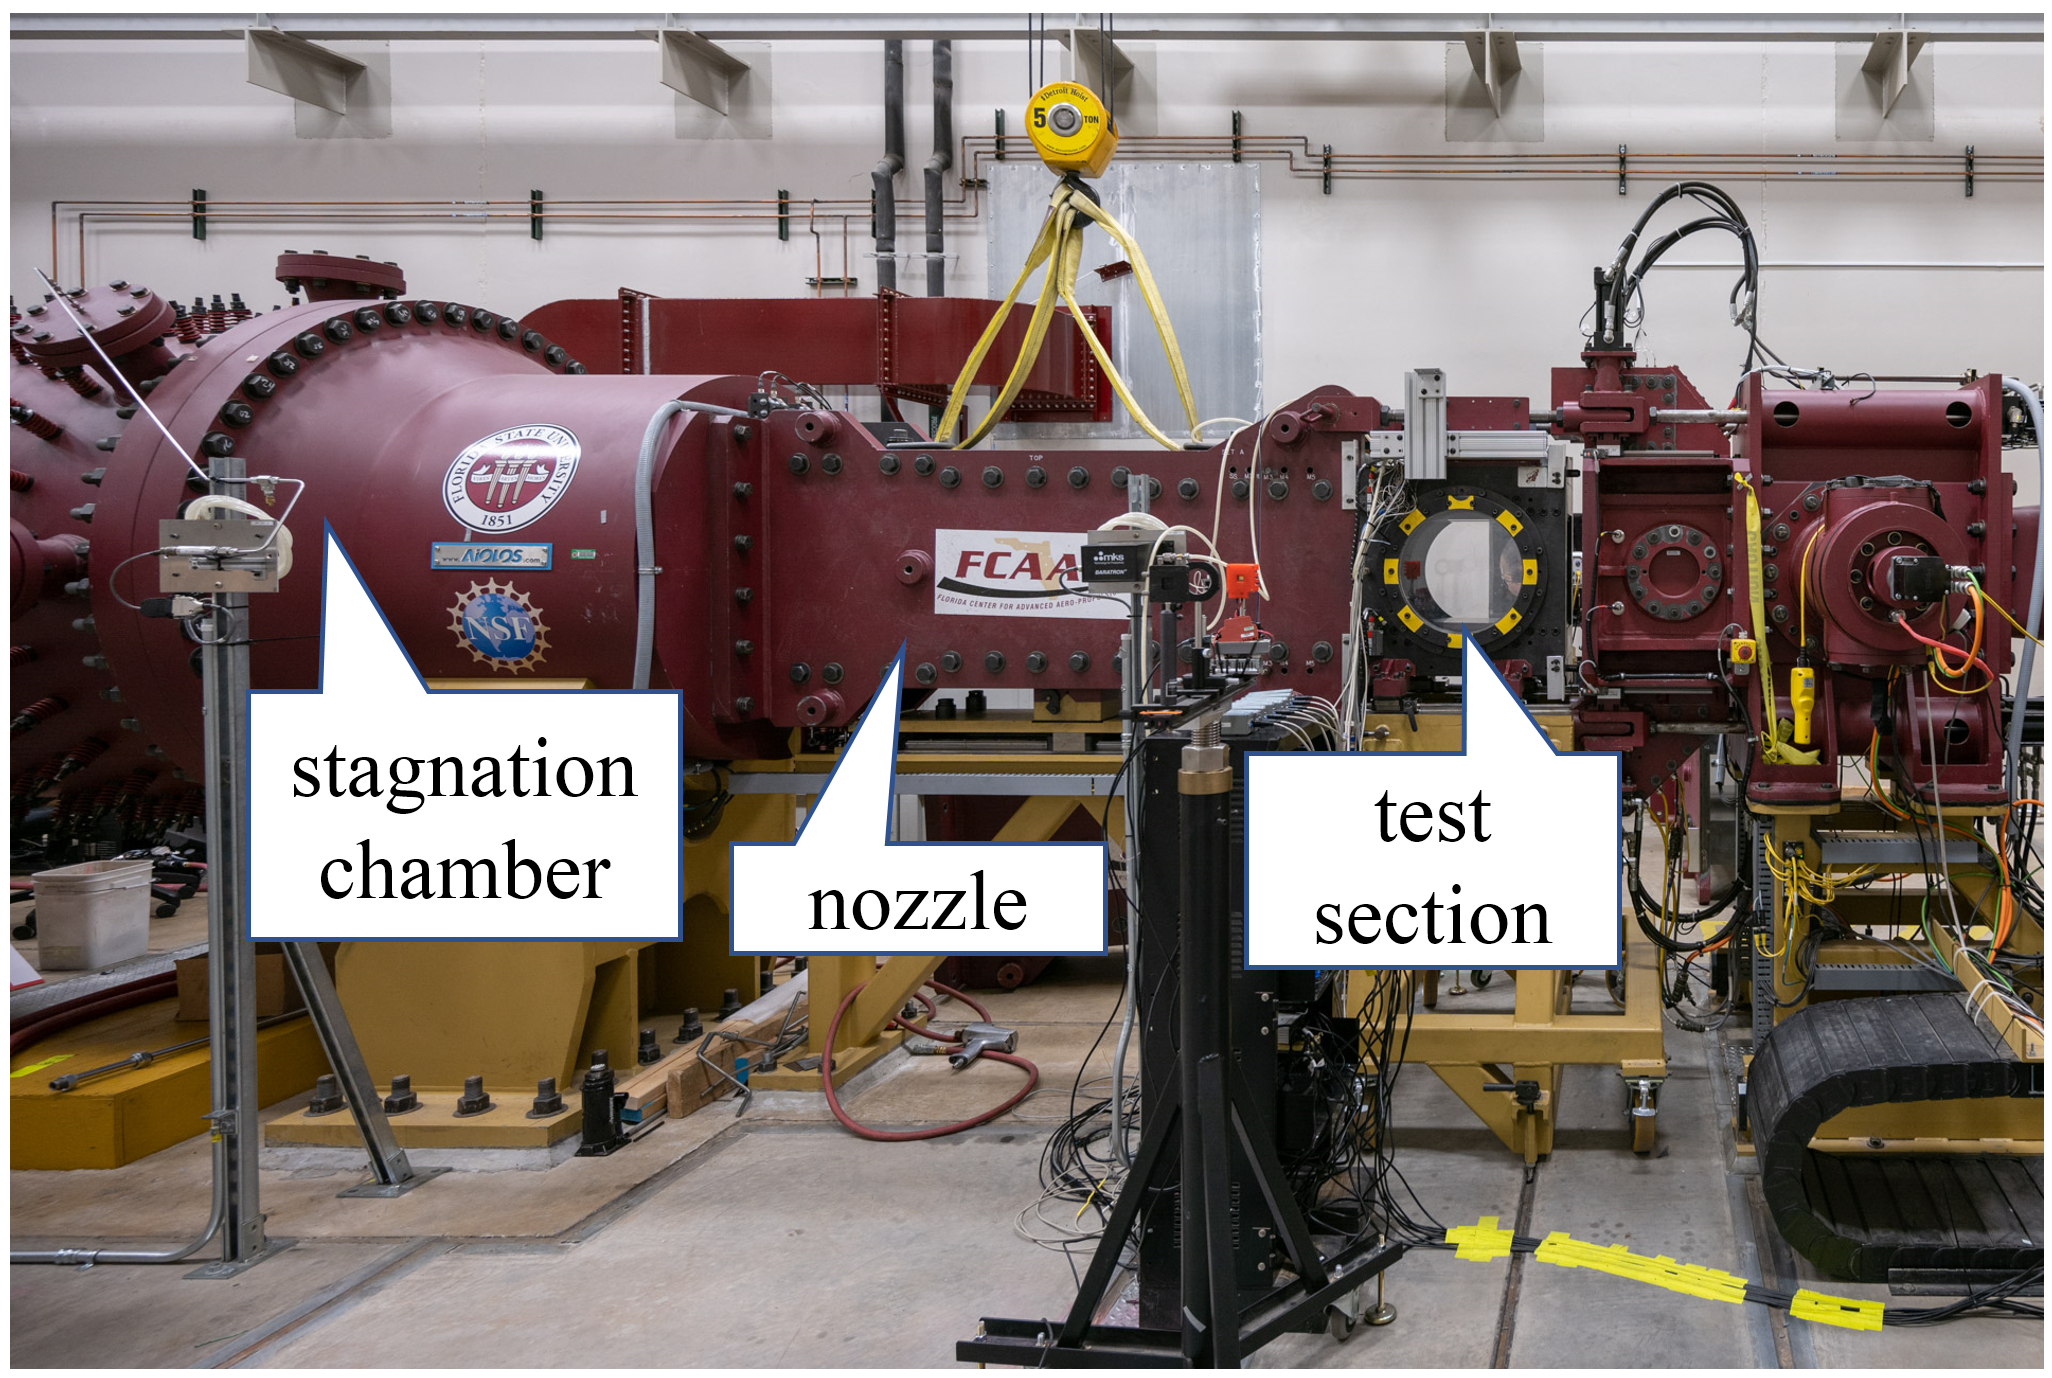
\includegraphics[width=0.5\linewidth]{./figures/fsu/PSWT.PNG}
    \caption{Polysonic Wind Tunnel at Florida State University}
    \label{fig:PSWT}
\end{figure}

The test campaign investigated shock-shock interactions generated by wedge shock generators with leading-edge deflections of $5^\circ$, $10^\circ$, and $15^\circ$. Each wedge had a 0.14 m span to balance 2D flow development with minimal blockage. The generators were mounted on diamond cross-section struts from the ceiling and floor, as illustrated in Fig.~\ref{fig:PIVsetup}. PIV measurements were performed in a vertical streamwise plane between the wedges, with a laser sheet introduced through the top of the test section. An Nd:YAG laser (EVG-200) operating at 7.23 Hz with 200 mJ/pulse and an inter-pulse delay of $0.8 \ \mu$s was used to illuminate the flow field. Two LaVision Imager Pro X cameras captured images from the side window: one wide-angle camera for the overall flow and one zoomed-in camera to capture the shock-shock interaction zone. The present study focuses on data from the \(10^\circ / 10^\circ\) wedge configuration at Mach 2.

\begin{figure}[ht!]
    \centering
    \includegraphics[width=0.5\linewidth]{./figures/fsu/PIVsetup.PNG}
    \caption{Test section side view showing shock generators on struts and the PIV laser sheet optics on top of the test section.}
    \label{fig:PIVsetup}
\end{figure}

Seeding for the PIV system was generated using a Wright nebulizer housed in a pressure vessel, shown in Fig.~\ref{fig:seedsystem}. The nebulizer used Rosco Fog Fluid, a glycol-based commercial seeding solution. Compressed air from the tunnel supply system was regulated to 0.55 MPa to drive the nebulizer. The air-seed mixture was introduced into the tunnel's stagnation chamber via a vertical seed pipe with five upstream-facing holes to ensure proper mixing. The long hose and pipe layout, however, may have affected the final particle size distribution due to settling of larger particles along the transport path.

\begin{figure}[ht!]
    \centering
    \begin{subfigure}{0.4\linewidth}
        \centering
        \includegraphics[width=0.6\linewidth]{./figures/fsu/Seeder_a.PNG}
        \caption{Wright nebulizer assembly removed from pressure vessel}
        \label{fig:wrightneb}
    \end{subfigure}%
    \hspace{0.05\linewidth}
    \begin{subfigure}{0.4\linewidth}
        \centering
        \includegraphics[width=0.6\linewidth]{./figures/fsu/Seeder_b.PNG}
        \caption{Seeder with air supply and outlet connected to stagnation chamber}
        \label{fig:seedcon}
    \end{subfigure}
    \caption{Seeding system used for PIV measurements in the Polysonic Wind Tunnel}
    \label{fig:seedsystem}
\end{figure}

\subsection{CFD data}
The CFD simulation was conducted using ANSYS 2021 R2. The initial grid of the domain under study to start the simulation is shown in Fig. \ref{fig:fsu_initial_grid}. The grid is refined in the shock interaction region to have a maximum cell thickness of $0.1mm$, totaling 33,097 cells. An adaptive mesh refinement strategy was utilized to capture the shock interaction region. The refinement is set to split the grid up to 8 levels of refinement using a gradient adaptation approach with a factor of 0.5. This process yielded a grid size of approximately $10^{-5} m$ in the shock cells. This final grid is shown in Fig. \ref{fig:fsu_final_grid}\par

\begin{figure}[ht!]
    \begin{subfigure}{0.5\linewidth}
        \centering
        \includegraphics[width=\linewidth]{figures/fsu/pdh/original_mesh_logo_removed.png}
        \caption{Initial grid}
        \label{fig:fsu_initial_grid}
    \end{subfigure}%
    \begin{subfigure}{0.5\linewidth}
        \centering
        \includegraphics[width=\linewidth]{figures/fsu/pdh/adapted_mesh_logo_removed.png}
        \caption{Final grid}
        \label{fig:fsu_final_grid}
    \end{subfigure}
    \caption{Initial and final grids to capture shock interaction for Mach 2 $10^\circ/10^\circ$}
    \label{fig:fsu_grids}
\end{figure}

The Reynolds-averaged Navier-Stokes (RANS) equations are solved using the \(k\)-\(\omega\) turbulence model, where \(k\) is the turbulence kinetic energy and \(\omega\) is the specific rate of dissipation of turbulence. This model is chosen due to its robustness in capturing regions with adverse pressure gradients.

In the Fluent solver, the operating pressure is set to 0~Pa. The boundary conditions are defined as follows:

\begin{itemize}
    \item \textbf{Inlet}: Set to pressure inlet. The gauge total pressure of 280,000~Pa, supersonic/initial gauge pressure of 35,785.27~Pa, and total temperature of 291.25~K.
    \item \textbf{Outlet}: Set to pressure outlet. The gauge pressure was 35,785.27~Pa.
    \item \textbf{Domain boundaries}: Set to far-field pressure conditions with a gauge pressure of 35,785.27~Pa.
    \item \textbf{Wedges}: The walls of the wedges are set to no-slip.
\end{itemize}

The velocity profile for the converged CFD data is shown in Fig.~\ref{fig:u_cfd}, while the corresponding PIV data is presented in Fig.~\ref{fig:u_piv}. The velocity contours are normalized by the free-stream velocity of 510~m/s. 

The PIV data is well-resolved, effectively capturing the incident shocks and their interaction region, which is the primary focus of this study. The regions with zero velocity in the PIV results are a consequence of experimental setup limitations, where optical constraints prevent data acquisition in those areas. The CFD data exhibits finer resolution due to the higher grid refinement, allowing for a more detailed representation of the flow structures.

\begin{figure}[hbt!]
    \begin{subfigure}{0.5\linewidth}
        \centering
        \includegraphics[width=\linewidth]{figures/fsu/pdh/u_contour_normalized.png}
        \caption{CFD}
        \label{fig:u_cfd}
    \end{subfigure}%
    \begin{subfigure}{0.5\linewidth}
        \centering
        \includegraphics[width=\linewidth]{figures/fsu/pdh/mach2_10-10_velocity_contour.png}
        \caption{PIV}
        \label{fig:u_piv}
    \end{subfigure}
    \caption{Normalized velocity contours for shock interaction case, Mach 2 $10^\circ/10^\circ$}
    \label{fig:shock_interaction_u_contours}
\end{figure}

%%%%%%%%%%%%%%%% 
%%%%%%%%%%%%%%%%
\section{Model Architecture}
The reduction in particle inertia bias in PIV images is a two-step problem. First, it inherently resembles optical flow estimation, where the goal is to predict the apparent motion of pixels between consecutive images. This is analogous to estimating the displacement of particle patterns between two snapshots of a flow field. Second, the particle motion deviates from the fluid motion due to particle inertia bias, which stems from differences in density, size, and response time of particles relative to the fluid. Correcting this bias involves tracking the particles and reconstructing the underlying flow field that the particles fail to represent accurately. This step requires understanding the dynamics of particle-fluid interactions, including drag forces, slip velocity, and the impact of flow gradients on particle behavior. Together, these two will drive the existing models to achieve a reduction in particle inertia bias in PIV images.

The bilateral CNN architecture implemented by Fan \emph{et al.} \cite{fan2023} for the intensity correction in PIV images is modified for the current implementation. Their model is designed to remove intensity noise in the PIV images. Their model features two encoders, a dual encoder, and two decoders that work in parallel to accept two PIV snapshots and remove intensity noise from them. The encoder-decoder networks have also demonstrated improved spatial resolution in velocity field computation for PIV images as studied by Yu \emph{et al.} \cite{yu2023}. One of the advantages of implementing a dual-encoder is that it can learn associated features of the input images simultaneously. Their model has been trained on about 7500 synthetic images. The results showed significant improvement to a maximum of 14.7\% compared to traditional techniques. However, this model is not complex enough to capture the optical flow component, which is a key requirement of this work.\par

To address this limitation, their bilateral CNN model's structure is enhanced with the U-Net architecture of Ronneberger \emph{et al.} \cite{ronneberger2015}, which enables hierarchical feature extraction and reconstruction. This architecture underlies several optical flow estimation models for PIV, as studied by Yu \emph{et al.} \cite{yu2023}. These models are specifically designed to capture dense motion fields and provide a robust foundation for modeling the optical flow component in PIV. By omitting pooling layers, as recommended by Fan \emph{et al.} \cite{fan2023}, the model retains critical features while leveraging the U-Net's ability to extract dense motion fields. This hybrid approach balances the strengths of bilateral CNNs and U-Net for improved particle inertia correction.\par

The bilateral CNN model effectively identifies artifacts in PIV images while preserving particle motion between frames, making it a strong foundation for our current approach. We hypothesize that this model can predict data with reduced inertia bias by incorporating information related to particle inertia. The bilateral model was chosen specifically for its ability to process two input images and output corresponding corrected images with reduced particle inertia bias. By operating directly on raw PIV images rather than processed data, the network focuses solely on correcting inertia bias without being influenced by other processing methods.\par

To achieve this, we modified the original bilateral CNN architecture to incorporate additional parameters that capture physics, such as freestream Mach and Reynolds numbers, which reflect particle and fluid properties. These scalar inputs provide the model with essential contextual information about particle-fluid dynamics, enabling more accurate correction of inertia bias while maintaining the architectural strengths of the bilateral CNN.\par

The Basset–Boussinesq–Oseen equation (BBO equation) gives the forces acting on a particle in a flow \cite{mei1996}. It is well understood that the drag force becomes the dominant force acting on a sub-micron particle traversing through a flow. Thus, the force per unit mass acting on a particle is given by Eq. \ref{eq:drag_equation}.

\begin{equation}
    \frac{d\boldsymbol{V}}{dt} = -\frac{3}{4} C_D Re_p \frac{\mu}{\rho_p {d_p}^2} (\boldsymbol{V} - \boldsymbol{U})
    \label{eq:drag_equation}
\end{equation}
%
where,\\
$C_D$ is the coefficient of drag, which is semi-empirical, \\
$Re_p$ is the particle Reynolds number, given by $\frac{\rho_f|V-U|d_p}{\mu}$, \\
$\mu$ is the dynamic viscosity of the fluid, \\
$V$, $U$ are the particle and fluid velocity magnitudes, respectively, and \\
$\boldsymbol{V}$, $\boldsymbol{U}$ are velocity vectors of the respective mediums.\\

Different drag coefficients are listed in Kalagotla \emph{et al.} \cite{kalagotla2024-aviation}. For the current work, the Loth drag model \cite{loth2008} is employed, as it has demonstrated consistent performance across various Mach regimes. This Loth drag model is a function of particle Reynolds number and particle Mach number, given by $M_p = \frac{|V- U|}{\sqrt{\gamma R T}}$, where $R$ is the gas constant, and $T$ is the static temperature. So, these parameters are needed as input for the machine learning model to conform to the bounds. Hence, the freestream Mach number and Reynolds number are added as input to the current model, as these are the parameters available during any PIV experiment. The Reynolds number is computed from the particle diameter. Thus, particle parameters are taken into account. Viscosity is calculated using Sutherland's law. After substituting and rearranging, the inputs to the model can be computed using Eq. \ref{eq:model_inputs}.\par

\begin{equation}
    Re = \sqrt{\frac{\gamma}{R}}\frac{\rho_f M d_p (T+S)}{C_1 T^2}
    \label{eq:model_inputs}
\end{equation}

Where $d_p$ is the particle diameter, $S = 110.4K$ is the Sutherland's constant, $C_1 = 1.458\times10^{-6} kg/m-s\sqrt{K}$

\begin{figure}[ht!]
\centering
    \includegraphics[scale=0.4]{figures/PIVnet_old.png}
    \caption{A schematic of the BICSNet}
    \label{fig:pivnet_architecture}
\end{figure}

The schematic for the network is shown in Fig. \ref{fig:pivnet_architecture}. The input images, each of shape $(256 \times 256 \times 3)$, are passed through a series of convolutional layers, followed by ReLU activation functions. These layers in the encoder extract low-level features such as edges, textures, and gradients, which are essential for identifying the basic structures in the images. As the data flows deeper into the network, the convolutional layers capture increasingly complex patterns, such as localized particle motion and interactions, which are critical for understanding the flow dynamics.

Once the features are extracted, they are passed through deconvolutional (transpose convolutional) layers in the decoder to reconstruct the corrected PIV images. This step ensures that the model retains spatial coherence while correcting particle inertia bias and aligning the outputs with the true flow field. Additionally, the scalar inputs — Mach and Reynolds numbers, computed based on the particle diameter — are introduced into the deep decoder layers. These inputs provide critical physical context, allowing the network to adapt the correction process to the specific flow conditions represented in the input data. This integration ensures that the model learns the image features and adheres to the underlying physics of the problem. However, unlike physics-informed neural networks (PINNs), this approach does not strictly enforce physical laws during the backpropagation process. This allows for greater flexibility while maintaining computational efficiency.\par

The current model employs sparse connections, whereas newer architectures may leverage denser networks or attention mechanisms to capture intricate interdependencies between features. This design choice reduces computational load, enhancing efficiency while maintaining accuracy in corrections. As Goodfellow \emph{et al.} \cite{goodfellow2016} highlighted, convolutional networks extract features hierarchically. The initial layers focus on pixel-level details, such as edges and corners, which are crucial for capturing the fine details of particles in PIV images. Subsequent layers aggregate these features into higher-order representations, such as particle clusters, localized flow structures, and larger-scale flow dynamics. This hierarchy enables the model to capture particle-level details and flow-field-level behaviors effectively. By selectively utilizing relevant information from the deeper encoder layers, the network focuses on particle inertia correction and optical flow estimation, ensuring that computational efficiency is balanced with the complexity required for accurate PIV image reconstruction.\par

Overall, the architecture combines convolutional feature extraction, scalar-based physical conditioning, and deconvolutional reconstruction to provide a robust framework for addressing particle inertia bias in PIV data.\par




%%%%%%%%%%%%%%%% 
%%%%%%%%%%%%%%%%
\section{Framework for Model Training and Testing}
This section presents a comprehensive framework for generating data on oblique shocks, designed to effectively train and test the model. The workflow process, as illustrated in Fig. \ref{fig:framework}, encapsulates three primary modules: Synthetic Data Generation, Input Data Preparation, and Model Parameter Optimization. Each module is critical in ensuring the performance of the model and is discussed in detail below.\par

\begin{figure}[ht!]
    \centering
    \includegraphics[width=\linewidth]{figures/framework.png}
    \caption{Framework for training and testing}
    \label{fig:framework}
\end{figure}

The synthetic data generation process, illustrated in Fig. \ref{fig:synthetic_data_generation}, integrates analytical or CFD flow data with particle dynamics to create high-fidelity datasets for training and testing the model. Flow fields are first generated on a computational grid, capturing the characteristics of oblique shocks. Particles with specified properties, such as size and density, are then traced through these fields using a one-way coupled Lagrangian Particle Tracking (LPT) code, which computes their trajectories. The code details are presented in Kalagotla \emph{et al.} \cite{kalagotla2023}. The resulting Lagrangian field is transformed into a Particle Dynamics History (PDH)-informed Eulerian field on a grid. The current work achieves this by sampling at least two data points in a cell and performing linear interpolation onto local nodes. This serves as a data reduction step, allowing us to generate several PIV-like images from a given flow field, assuming the underlying flow is steady-state. These fields are fed into a synthetic image generator, which produces 128 sets of images per case, each consisting of a first snapshot and two consecutive second snapshots derived from the PDH-informed and CFD data. This process ensures the synthetic images replicate real-world conditions, enabling the model to learn and predict particle-flow interactions in complex shock environments.\par

The input data preparation module is the second aspect in Fig. \ref{fig:framework}. Particle dynamics inform the input images. These are generated using the process described above. The freestream Mach number is the associated Mach number for each flow field, and the Reynolds number can be computed using Eq. \ref{eq:model_inputs}.\par

\begin{figure}[ht!]
    \centering
    \includegraphics[width=1.0\linewidth]{figures/synthetic_data_generation.png}
    \caption{Synthetic Data Generation to capture particle inertia bias with interrogation area highlighted}
    \label{fig:synthetic_data_generation}
\end{figure}

Finally, the model parameters are optimized in the highlighted Model parameter optimization module in Fig. \ref{fig:framework}. BICSNet parameters are optimized using the Adam optimizer \cite{kingma2014} and the Mean Squared Error (MSE) loss function. The MSE loss quantifies the error between the predicted and ground-truth images, defined as the average of squared differences, given by Eq. \ref{eq:mse}. The Adam optimizer combines momentum and adaptive learning rates, dynamically adjusting parameter updates based on first- and second-moment estimates of gradients, allowing for efficient and stable convergence even with sparse and high-dimensional data, such as PIV. These optimization methods are crucial for understanding various aspects of the flow fields.\par

\begin{equation}
    loss = \frac{1}{m}\frac{1}{n}\sum_{i=1}^{m}\sum_{i=1}^{n}(I_{truth}(i, j) - I_{pred}(i, j))^2
    \label{eq:mse}
\end{equation}
%
where,\\
$m, n$ are the dimensions of the image\\
$I_{truth}(i, j)$ is the pixel intensity at $(i, j)$ in the ground truth or label image\\
$I_{pred}(i, j)$ is the pixel intensity at $(i, j)$ in the model predicted image\\


\subsection{Details of the Dataset}
 The range of shock strengths chosen for this study can be understood from Fig. \ref{fig:shock_chart}. The training data set is generated at four different Mach numbers that are unevenly distributed. Three deflection angles were chosen for each Mach number. This data is highlighted in the figure. The testing dataset is created at two different Mach numbers with three different deflection angles, which account for two different shock strengths. The flow field is randomly generated by randomly choosing temperature and pressure typical of real PIV experiments.\par

\begin{figure}[ht!]
    \centering
    \includegraphics[width=0.7\linewidth]{figures/oblique_chart_training_testing_data.png}
    \caption{Range of Mach and deflection angles used for training and testing the BICSNet}
    \label{fig:shock_chart}
\end{figure}

At each point in Fig. \ref{fig:shock_chart}, five different particle diameters and densities were chosen that are typical of particle distributions found in the PIV experiments. The inputs for flow generation are presented in Table \ref{tab:flowfield_dataset}. Finally, for the ease of data generation and control, the oblique shock is aligned with the Cartesian grid so that the inlet flow velocity is horizontal.\par

\begin{table}[ht!]
\caption{Description of the flow fields generated for training and testing the BICSNet.}\label{tab:flowfield_dataset}
\begin{tabular}{@{}lll@{}}
\toprule
\textbf{Parameter} & \textbf{Training Set} & \textbf{Testing Set} \\
\midrule
Mach Number           & 1.5, 3.0, 4.3, 5.0    & 2.5, 7.6             \\
Deflection Angles     & 3 distinct values     & 3 distinct values    \\
Shock Strength        & Weak/Strong           & Weak/Strong          \\
Temperature           & Randomly chosen       & Randomly chosen      \\
Pressure              & Randomly chosen       & Randomly chosen      \\
Particle Diameter     & 5 distinct values     & 5 distinct values    \\
Particle Density      & 5 distinct values     & 5 distinct values    \\
Total no. of datasets & 600                   & 300                  \\
\botrule
\end{tabular}
\end{table}



The image generation parameters are also varied to account for the realistic conditions in PIV. At each training data point in Fig. \ref{fig:shock_chart}, the parameters are listed in Table \ref{tab:imagegen_dataset}. The particle diameters and densities are varied to capture a range of particle dynamics and inertia bias for each oblique shock case. The particle concentration varies between 0.03 and 0.06 particles per pixel, capturing typical particle densities in the interrogation windows of supersonic PIV experiments. Similarly, the percentage of in-plane particles also varies. The laser properties are all kept constant. The camera settings, such as the magnification and pixel resolution, are kept steady and are handled by varying domain settings that also affect the shock location. For example, magnification can be adjusted by keeping the shock location constant and varying the bounds of the interrogation area. Finally, particle distribution throughout the domain is uniform. These conditions provide a diverse dataset representation for the model to learn effectively for various oblique shocks.\par

% Please add the following required packages to your document preamble:
% \usepackage{multirow}
\begin{table}[ht!]
\caption{Description of the image generation parameters for training and testing the BICSNet.}
\label{tab:imagegen_dataset}
\centering
\begin{tabular}{@{}llp{0.5\linewidth}@{}} % relative width instead of 8.2cm
\toprule
\textbf{Category} & \textbf{Parameter} & \textbf{Values/Description} \\
\midrule
\multirow{5}{*}{Particle Specs} 
  & Particle Diameter         & Multiple diameters (0.5~$\mu$m, 5~$\mu$m, 10~$\mu$m, 30~$\mu$m, 40~$\mu$m) \\
  & Particle Density          & Multiple densities (950, 1212.5, 1475, 1735.5, 2000~kg/m$^3$) \\
  & Concentration             & Gaussian, log-normal distribution (0.03--0.06 per pixel) \\
  & Shape                     & Fixed -- Spherical \\
  & In-plane percent          & Variable (75--95\%) \\
\midrule
\multirow{4}{*}{Laser Properties} 
  & Laser thickness           & Fixed value (1~mm) \\
  & Pulse timing              & Fixed time delay, $\Delta t = 1~\mu$s \\
  & Domain location           & Fixed \\
  & Intensity distribution    & Fixed -- Gaussian \\
\midrule
Domain Settings 
  & Shock Location            & Algorithmically varied positions (e.g., mid-domain, near edges) \\
\midrule
Distribution Settings 
  & Particle Distribution     & Fixed -- Uniform \\
\midrule
\multirow{2}{*}{Imaging Properties} 
  & Magnification             & Varies with domain size \\
  & Pixel Resolution (dx)     & Fixed \\
\botrule
\end{tabular}
\end{table}


%%%%%%%%%%%%%%%% 
%%%%%%%%%%%%%%%%
\section{Model Evaluation}
The results of this study are presented in terms of the training process, validation performance, and the final evaluation of the testing dataset. These metrics were carefully analyzed to assess the ability of the current model to generalize and effectively correct particle inertia bias.\par

\subsection{Training and Evaluation of BICSNet}
BICSNet was trained on a dataset described in the previous section, split into 70\% training, 15\% validation, and 15\% testing. The training employed a learning rate of $10^{-4}$, with a decay factor of 0.8 triggered by patience of 2, meaning the learning rate was reduced after two consecutive epochs of an increasing validation error. The training process was monitored using loss metrics, which were logged at each iteration and epoch. Additionally, sample outputs were generated and visualized every 100 iterations within each epoch to evaluate qualitative progression. A sample taken during the late training is shown in Fig. \ref{fig:training_progress}. The figure displays relevant information, including the current learning rate, training loss, and scalar values. For example, this sample was generated for a Mach 5 case. The remaining values, such as epochs, validation loss, and training loss, are static. The predicted snaps from the model are shown on the left side, and true snaps are displayed on the right side of the figure. A small red circle is randomly generated to visually check the locations.\par

\begin{figure}[ht!]
    \centering
    \includegraphics[width=\linewidth]{figures/training_progress.png}
    \caption{Random sample generated during training to visually track the training progress}
    \label{fig:training_progress}
\end{figure}

The model achieved convergence on the validation set with a mean squared error (MSE) of $2.34 \times 10^{-4}$ after 77 epochs, trained using a batch size of 36 on four NVIDIA H100 GPUs at UC Advanced Research Computing (ARC) \cite{arc2019}. GPU memory utilization averaged 85\% across three GPUs and peaked at 98\% on the fourth GPU throughout training. Each epoch required approximately 3 GPU hours, resulting in a total training time of about 11 days, including validation computations between epochs. 

The final evaluation of the test set yielded an MSE of $2.20 \times 10^{-4}$, indicating robust generalization and alignment between training, validation, and testing performance. This suggests that the model effectively captures and corrects the particle inertia bias inherent in the dataset.

\subsection{Error metric}
The image pairs are analyzed using openPIV \cite{liberzon2020}. A 32x32 interrogation window is used by default with 75\% overlap to explore all the datasets. The data is averaged over 128 image pairs obtained for each case, and the error is computed using the L2-norm of the velocity fields. This is given by Eq. \ref{eq:l2-norm}.

\begin{equation}
    ||V_{n} - V_{truth}||_2 = \sqrt{\sum_{i=1}^{N} (V_{n,i} - V_{truth, i})^2} \quad \forall \quad n \in (model, input)
    \label{eq:l2-norm}
\end{equation}

Where $V$ is the normalized shock-normal velocity.\par

A sample data highlighting the normalized shock-normal velocity vs. the normalized shock-normal distance is shown in Fig. \ref{fig:error_metric}. The plot highlights the error metric between model-to-truth and input-to-truth. All of the relevant parameters are highlighted in the title of the figure.\par

\begin{figure}[ht!]
    \centering
    \includegraphics[width=0.7\linewidth]{figures/error_metric.png}
    \caption{Error metric from a sample}
    \label{fig:error_metric}
\end{figure}

\subsection{Testing the model performance}
As described in the previous section, the model's performance is evaluated on a different test set. This section examines the error metric across the entire test set. Later, each relevant parameter is isolated, and the model's performance is understood for each parameter.

\subsubsection{Error analysis}
A new image set is generated using all the variables in the training set for the flowfield. The shock location is kept consistent at each data point in Fig. \ref{fig:shock_chart}, and image generation parameters are varied to generate the testing image set for flow parameters included in the training of the model. This allows us to replicate real-world scenarios of studying oblique shocks.\par

The error distribution between Input-to-Truth (left) and Model-to-Truth (right) for the whole dataset, including flow parameters from the training set and testing set, are shown in Fig. \ref{fig:error_distribution}. The Input-to-Truth error exhibits a nearly uniform distribution, with a notable peak at the lowest end, suggesting that the error is minimal for most cases. This behavior highlights the inherent quality of the synthetic PIV (syPIV) data as a baseline. On the other hand, the Model-to-Truth error distribution shows a significant reduction in the average error of approximately 83\% compared to the Input-to-Truth error, dropping from 1.35 to 0.23. Despite this improvement, the Model-to-Truth error distribution has more significant outliers, indicating that while the model effectively reduces the overall error, specific predictions still exhibit substantial discrepancies.\par

Additionally, the spread of errors is slightly narrower for the Model-to-Truth distribution (0.78) compared to the Input-to-Truth (0.81), suggesting a moderate improvement in consistency. This comparison highlights the model's ability to effectively correct particle inertia bias while identifying areas where further refinement is needed to address outlier errors. This can be further analyzed by looking at independent Mach numbers to understand where the significant error is generated.\par

\begin{figure}[ht!]
    \centering
    \includegraphics[width=\linewidth]{figures/error_analysis/error_distribution.png}
    \caption{Error distribution for the whole dataset}
    \label{fig:error_distribution}
\end{figure}

Further, when only the Mach numbers included in the training set are considered, the distribution is shown in Fig. \ref{fig:error_distribution_training}. The Input-to-Truth error distribution (left) maintains a similar pattern to the overall dataset, showing a nearly uniform distribution with a peak at lower error values. The Model-to-Truth error distribution (right) demonstrates a significant reduction in average error, decreasing by 87\%, from 1.34 to 0.17. This highlights the model's effectiveness in learning from the training dataset to correct particle inertia bias.\par

\begin{figure}[ht!]
    \centering
    \includegraphics[width=\linewidth]{figures/error_analysis/error_distribution_training.png}
    \caption{Error distribution for the training Mach numbers}
    \label{fig:error_distribution_training}
\end{figure}

Additionally, the spread in errors narrows from 0.77 to 0.56, signifying an improvement in consistency across the dataset. Unlike the results for the entire dataset, model predictions for the training Mach numbers are as good as or better than the Input data, with fewer significant outliers. This outcome suggests that the model performs exceptionally well when applied to scenarios similar to its training conditions, affirming its reliability in such cases.\par

For the in-distribution Mach 2.5 case, highlighted in Fig. \ref{fig:shock_chart}, the error distribution is shown in Fig. \ref{fig:error_distribution_testing_2.5}. This depicts the error distributions for a Mach number excluded from the training set. The Input-to-Truth error distribution (left) shows a relatively uniform pattern, with a peak at the lowest end, indicating minimal error for most cases in the syPIV data. The Model-to-Truth error distribution (right) reveals an average error reduction of 78\%, from 0.86 to 0.19, demonstrating the model's capability to generalize to unseen scenarios. However, the spread increases from 0.69 to 0.89, reflecting a 29\% rise, which indicates more significant prediction variability, including some incorrect cases. Significant outliers corroborate this behavior in the Model-to-Truth error distribution, where specific predictions exhibit larger discrepancies than the syPIV data. These results align with the observations for the overall dataset, highlighting that while the model effectively reduces the average error, its predictions for unseen conditions exhibit higher variability and occasionally significant errors. This suggests that the model can be improved for the cases not included in the training, which can be achieved by improving the model with physics-based optimization techniques.\par

\begin{figure}[ht!]
    \centering
    \includegraphics[width=\linewidth]{figures/error_analysis/error_distribution_testing_2.5.png}
    \caption{Error distribution for the in-distribution Mach 2.5 case}
    \label{fig:error_distribution_testing_2.5}
\end{figure}

Finally, for the Mach 7.6 case, which is out-of-distribution of the Mach numbers used in the training process, the error distribution is shown in Fig. \ref{fig:error_distribution_testing_7.6}.  The Input-to-Truth error distribution (left) has an average error of 1.81 and a standard deviation of 0.80, indicating a non-uniform distribution with a significant peak at higher error values, which suggests larger errors in the syPIV data for this case. This is typical for high supersonic flows. The Model-to-Truth error distribution (right) reduces the average error by only 30\%, from 1.81 to 1.27. However, the spread increases by 27\%, from 0.80 to 1.02, suggesting higher variability in model predictions. The presence of significant outliers in the Model-to-Truth distribution suggests that the model struggles to generalize effectively at this high Mach number, resulting in more pronounced errors than the syPIV baseline. This suggests that the model demonstrates limited effectiveness in reducing errors under conditions significantly different from those used in training.\par

\begin{figure}[ht!]
    \centering
    \includegraphics[width=\linewidth]{figures/error_analysis/error_distribution_testing_7.6.png}
    \caption{Error distribution for the out-of-distribution Mach 7.6 case}
    \label{fig:error_distribution_testing_7.6}
\end{figure}

\begin{comment}
\subsubsection{Error to parameter correlation analysis}
The correlation between model-to-truth error and critical parameters, including Mach number, deflection angle, mean particle diameter, and particle density, reveals vital insights into the model's performance and areas for further improvement. Figure \ref{fig:correlation-1} highlights these relationships, showcasing trends that underline the complexities associated with each parameter.

\begin{figure}[ht!]
    \centering
    % Top-left subfigure
    \begin{subfigure}[b]{0.45\textwidth}
        \centering
        \includegraphics[width=\textwidth]{figures/correlation-1/error_vs_mach.png}
        \caption{Model-to-Truth Error vs. Mach numbers}
        \label{fig:error_vs_mach_correlation}
    \end{subfigure}
    % Top-right subfigure
    \begin{subfigure}[b]{0.45\textwidth}
        \centering
        \includegraphics[width=\textwidth]{figures/correlation-1/error_vs_deflection.png}
        \caption{Model-to-Truth Error vs. Deflection angles}
        \label{fig:error_vs_deflection_correlation}
    \end{subfigure}
    \\ % Line break for next row
    % Bottom-left subfigure
    \begin{subfigure}[b]{0.45\textwidth}
        \centering
        \includegraphics[width=\textwidth]{figures/correlation-1/error_vs_dp_mean.png}
        \caption{Model-to-Truth Error vs. Mean particle diameters}
        \label{fig:error_vs_dp_mean_correlation}
    \end{subfigure}
    % Bottom-right subfigure
    \begin{subfigure}[b]{0.45\textwidth}
        \centering
        \includegraphics[width=\textwidth]{figures/correlation-1/error_vs_rhop.png}
        \caption{Model-to-Truth Error vs. Particle densities}
        \label{fig:error_vs_rhop_correlation}
    \end{subfigure}

    \caption{Correlation analysis between Model-to-Truth error vs. parameters of significance}
    \label{fig:correlation-1}
\end{figure}

As the Mach number increases, the model-to-truth error exhibits an upward trend, as shown in Figure \ref{fig:error_vs_mach_correlation}. This behavior aligns with expectations, given the higher levels of lag experienced by particles associated with stronger shocks at higher Mach numbers. However, this trend aggregates results across all shock strengths at each Mach number, masking some behavior. Notably, the model demonstrates significant potential for improvement as shock strength increases, particularly at extreme Mach values, where errors are most pronounced.\par

The deflection angle presents a slightly different relationship with the model-to-truth error, as illustrated in Figure \ref{fig:error_vs_deflection_correlation}. A slight negative slope compared to the Input-to-Truth error indicates that the error decreases marginally as the deflection angle increases. This trend may reflect the model's ability to generalize better for higher deflection angles under certain conditions. However, localized increases in error are evident at specific deflection angles, particularly for a Mach number of 7.6, which is an out-of-distribution case. These anomalies highlight areas where the model could benefit from additional training data or refined architecture adjustments to capture the underlying physics more accurately.\par

The relationship between mean particle diameter and model-to-truth error, depicted in Figure \ref{fig:error_vs_dp_mean_correlation}, shows an apparent increase in error with larger particle diameters. While input-to-truth and model-to-truth errors follow this trend, the slope for the model-to-truth error is noticeably less steep. This reduced slope indicates the model's ability to mitigate the impact of increasing particle size on error, which is a desirable outcome. Further data for particle sizes not included in the training set is being generated, providing additional validation and insights into the model's robustness across particle size variations.\par

Finally, particle density exhibits the least influence on model-to-truth error, as evident from the near-flat slope in Figure \ref{fig:error_vs_rhop_correlation}. Unlike parameters such as Mach numbers, particle density is not directly used during training, which may explain its minimal effect on error trends. This insensitivity suggests that the model can effectively generalize across variations in particle density, a promising outcome for broader applications.\par
\end{comment}

\begin{comment}
\subsubsection{Error reduction correlation analysis}
The error reduction based on the parameter of interest could be understood by the amount of correlation between Model-to-Truth vs. Input-to-Truth error plots for a given parameter. This section explores how each parameter affects the model's performance.\par

For each Mach number, the correlation between the errors is shown in Fig. \ref{fig:correlation_mach}. This analysis highlights the error reduction achieved by the model for each Mach number. In an ideal scenario, a horizontal line at zero would signify perfect model predictions, indicating no residual error between the predicted and true values. Consequently, lower Pearson correlation coefficients and narrow confidence intervals indicate effective error mitigation. The data suggests that this desirable trend is predominantly observed, except for Mach 1.5, which shows minimal improvements in error.\par

\begin{figure}[ht!]
    \centering
    \includegraphics[width=\linewidth]{figures/correlation-2/correlation_mach.png}
    \caption{Correlation between errors at each Mach number in the dataset}
    \label{fig:correlation_mach}
\end{figure}

Furthermore, the results for Mach numbers not included in the training data demonstrate higher variance, as evident from the wider confidence intervals. This behavior underscores the challenges the model faces when extrapolating beyond the training set. These findings emphasize the importance of incorporating diverse training data to enhance the model's robustness and generalization capabilities.\par

Figure \ref{fig:correlation_deflection} illustrates the relationship between input-to-truth and model-to-truth errors for varying Mach numbers and deflection angles, arranged by increasing shock strength from top to bottom. The lower correlation coefficients (r-values) between input-to-truth and model-to-truth errors indicate better model performance. This behavior suggests that even when input-to-truth errors are high, the model effectively reduces the model-to-truth error.\par

The data reveals that stronger shocks, which inherently introduce more significant initial errors, exhibit lower r-values and, thus, better error correction. For instance, at higher shock strengths (bottom rows of the figure), the model significantly reduces model-to-truth errors, where input-to-truth errors are high. This trend highlights the model’s ability to make corrections in flow regimes where the initial predictions deviate significantly from the actual values.\par

\begin{figure}[ht!]
    \centering
    \includegraphics[width=\linewidth]{figures/correlation-2/correlation_deflection.png}
    \caption{Correlation between errors at each deflection angle in the dataset}
    \label{fig:correlation_deflection}
\end{figure}

At specific Mach-deflection combinations, variability in r-values highlights regions for potential improvement. For example, at Mach 4.3 with a deflection angle of $26.42^o$, the r-value is notably low (r=0.10), reflecting an excellent reduction in error. Conversely, at weaker shocks and lower deflection angles, r-values are higher, indicating that the model's corrections are less pronounced due to lower initial errors and less room for improvement.\par

These findings highlight the model’s strengths in addressing high-error scenarios in the presence of strong shocks. They also highlight the need for expanding training data in regimes where corrections are less effective to ensure consistently low model-to-truth errors across all Mach and deflection angle combinations.\par

\begin{figure}[ht!]
    \centering
    \includegraphics[width=\textwidth]{figures/correlation-2/correlation_particle_diameters.png}
    \caption{Correlation between errors for different particle diameters.}
    \label{fig:correlation_particle_diameters}
\end{figure}

Fig. \ref{fig:correlation_particle_diameters} explores the relationship between input-to-truth and model-to-truth errors for different particle diameters. The correlation coefficients (r-values) remain relatively consistent across all diameters, with minor variations highlighting specific trends. Notably, the smallest diameter ($0.5 \mu m$) exhibits the highest r-value ($r=0.85$), suggesting a stronger linear relationship between input and model errors for this diameter. This observation suggests that the model's corrective capabilities are less pronounced at smaller diameters, where initial errors are likely to be smaller.\par

A closer inspection reveals that most data is skewed toward smaller error values, resulting in tighter confidence intervals (CI) in these regions. However, at larger error magnitudes, the confidence interval (CI) spread increases significantly, indicating reduced confidence in the model's predictions for outliers or extreme cases. This shows an area for improvement where more training data could be generated for cases with high Input-to-Truth errors.\par

The consistency in r-values across diameters suggests that the model generalizes well across different particle sizes. This analysis highlights the need for targeted improvements in the model architecture or training set to address scenarios involving larger particle diameters with high initial errors.

\begin{figure}[ht!]
    \centering
    \includegraphics[width=\textwidth]{figures/correlation-2/correlation_particle_densities.png}
    \caption{Correlation between errors for different particle densities.}
    \label{fig:correlation_particle_densities}
\end{figure}

Fig. \ref{fig:correlation_particle_densities} highlights the relationship between input-to-truth and model-to-truth errors for varying particle densities. The results indicate that particle density has a relatively uniform effect on error correction, with correlation coefficients (r-values) remaining consistent across all densities. The values range between $r=0.53$ and $r=0.61$, showing minimal variability. This suggests that the model generalizes well across different densities and is not significantly influenced by variations in this parameter.\par

The narrow confidence intervals across most error ranges further emphasize the model's reliability in handling density variations. However, the confidence intervals are slightly widening at larger Input-to-Truth error values. This indicates reduced confidence in predictions for outliers or extreme cases but does not significantly impact the overall performance trends.\par

The uniformity in r-values and the minimal impact of density on error correction demonstrate the robustness of the model when applied to data with varying particle densities. These results highlight the model's ability to decouple particle density effects from error predictions, further supporting its generalization capabilities.\par


\end{comment}

\begin{comment}
\subsubsection{Peak Signal-to-Noise ratio}
The Peak Signal-to-Noise Ratio (PSNR) is a widely used metric for assessing the quality of image reconstruction or prediction by comparing a predicted image to its ground-truth counterpart. Defined mathematically in Eq. \ref{eq:psnr}, PSNR quantifies the degree to which the model retains essential image features while minimizing distortions caused by noise or errors. A higher PSNR value indicates better model performance, signifying a closer alignment between the predicted and actual data. This makes PSNR a critical tool for evaluating whether the reconstructed features accurately preserve the underlying physics, ensuring that physical phenomena remain unchanged during prediction.

\begin{equation}
    PSNR = 10 \times log_{10}\biggl(\frac{MAX^2}{MSE}\biggr)
    \label{eq:psnr}
\end{equation}
%
where,\\
$MAX$ is the maximum possible intensity value for the image. For the current case, it is 255.\\
$MSE$ is the mean squared error between image intensities and can be computed using Eq. \ref{eq:mse}.\par

\begin{figure}[ht!]
    \centering
    \includegraphics[width=\linewidth]{figures/psnr/psnr_distribution.png}
    \caption{PSNR distribution for Input-to-Truth and Model-to-Truth}
    \label{fig:psnr_distribution}
\end{figure}

Figure \ref{fig:psnr_distribution} presents the PSNR distributions for the model predictions compared to the input data. The Input-to-Truth PSNR distribution (left) has a median of 38.04 and a spread of 10.55, showing a wide range as expected due to the particle inertia bias, which is almost negligible for low shock strengths and small particle diameters. In contrast, the Model-to-Truth PSNR distribution (right) exhibits a slightly higher median of 38.95 with a significantly reduced spread of 4.23, indicating more consistent predictions. The left-skewed nature of the Model-to-Truth distribution further demonstrates that the network performs better in most cases. However, the reduction in high PSNR values, which typically correspond to low shock strengths and smaller particle diameters, highlights a limitation in the network's ability to generalize to these conditions. This shortcoming is likely due to the absence of skip connections, which can better retain fine-grained features critical for high-accuracy predictions. Future work will incorporate skip connections and denser implementations to enhance the generalization capabilities of the network and address this limitation.\par

\begin{figure}[ht!]
    \centering
    \includegraphics[width=0.7\linewidth]{figures/psnr/psnr_analysis.png}
    \caption{PSNR analysis per parameter for Input-to-Truth and Model-to-Truth}
    \label{fig:psnr_analysis}
\end{figure}

Figure \ref{fig:psnr_analysis} illustrates the PSNR trends across different parameters for the model predictions. While the network generalizes well for intermediate Mach numbers, its performance declines sharply for low and high Mach numbers, particularly at Mach 7.6, where PSNR values are significantly lower. Similarly, the Model-to-Truth PSNR decreases notably for smaller particle diameters, indicating challenges in capturing the fine-scale features associated with such cases. On the other hand, particle density shows consistent trends, with only a slight drop in PSNR as density increases, suggesting that the network is robust to variations in this parameter.\par

The deflection angle introduces substantial variability in Input-to-Truth PSNR, but the Model-to-Truth PSNR remains comparatively stable across different angles, albeit at a lower overall level. This stability highlights the network's reduced sensitivity to this parameter, indicating room for improvement in prediction accuracy. These trends suggest that the current network architecture struggles with extreme cases and fine-grained details, necessitating future enhancements such as skip connections to improve generalization and capture finer-scale information.\par

Finally, the consistent performance for particle density and intermediate Mach numbers underscores the model's potential for robust predictions under specific conditions, with opportunities for further optimization.\par

\end{comment}
%%%%%%%%%%%%%%%% 
%%%%%%%%%%%%%%%%
\section{Application to Experimental PIV Data}
In this section, the Mach 2 $10^\circ/10^\circ$ shock-interaction data set is used to demonstrate the efficacy of BICSNet on experimental PIV data. This dataset comprises 365 particle image pairs captured by a 2048$\times$2048 pixel camera. The current machine learning model has been trained on a synthetic dataset containing a single oblique shock aligned with the Cartesian grid, with assumptions of uniform particle seeding, fixed laser pulse timing, and constant magnification. It is essential to pre-process the experimental PIV data to enable BICSNet to extract meaningful features and correct for particle inertia bias. This pre-processing aims to minimize the shift in intensity distribution compared to the synthetic data for training the BICSNet model.

\subsection{Pre-processing PIV data to work with BICSNet}\label{sec:preprocesing}
Since the machine learning model was trained on cases where the oblique shock was aligned with the Cartesian grid, the PIV data obtained from the shock interaction experiments were modified by rotating and cropping the incident shock region, as illustrated in Fig.~\ref{fig:bicsnet_cropped_image}.

\begin{figure}[ht!]
    \centering
    \includegraphics[width=\linewidth]{./figures/06pivnet/piv/preview.png}
    \caption{Steps to isolate the incident shock region from shock-interaction PIV image}
    \label{fig:bicsnet_cropped_image}
\end{figure}

To process the full shock interaction data obtained from the PIV experiments, each 2048$\times$2048 pixel image containing the shock interaction was cropped into 256$\times$256 pixel patches with a 50\% overlap. This procedure produced 225 cropped images per PIV frame, as shown in Fig.~\ref{fig:shock_interaction_crops}. In this figure, 128$\times$128 pixel regions are outlined, with four such regions composing a single 256$\times$256 pixel image patch. This patching structure is further highlighted using a red square in Fig.~\ref{fig:256px_grid}, with the corresponding extracted patch shown in Fig.~\ref{fig:256px_crops}. Each cropped image was then pre-processed to match the intensity levels of the synthetic training data described below. In total, 94,095 image pairs generated through this process were processed using the BICSNet model to correct for particle inertia bias.
\par

Since the BICSNet model was trained on synthetic oblique shocks aligned with the Cartesian grid, the shock regions in the experimental shock interaction data were reprocessed by rotating the images, as shown in Fig.~\ref{fig:bicsnet_cropped_image}, with a 50\% overlap. This procedure resulted in a total of 5,475 image pairs. This data set also consists of two image pairs with shock interaction regions, an out-of-distribution case for the current model based on flow features.\par

\begin{figure}[ht!]
    \centering
    % Top-left subfigure
    \begin{subfigure}[b]{0.45\textwidth}
        \centering
        \includegraphics[width=\textwidth]{./figures/06pivnet/piv/256px_grid.png}
        \caption{2048$\times$2048 pixel image from PIV}
        \label{fig:256px_grid}
    \end{subfigure}
    % Top-right subfigure
    \begin{subfigure}[b]{0.45\textwidth}
        \centering
        \includegraphics[width=\textwidth]{./figures/06pivnet/piv/256px_crops.png}
        \caption{256$\times$256 px patches with 50\% overlap}
        \label{fig:256px_crops}
    \end{subfigure}

    \caption{Procedure to process experimental PIV data using BICSNet}
    \label{fig:shock_interaction_crops}
\end{figure}

Further, the intensity distributions between the PIV and synthetic images significantly differ, as seen in Fig. \ref{fig:bicsnet_synthetic_vs_cropped}. The figure compares the intensity data between the synthetic and the cropped experimental PIV images at the incident shock location. The experimental PIV images have a high proportion (approximately 80\%) of black levels or zero pixels, as indicated by the intensity frequency plot, compared to the synthetic image, which also has a significant proportion (approximately 25\%) of zero pixels but a continuous distribution of low-intensity pixels. The synthetic images are generated with a uniform particle distribution, an ideal case for experimental PIV images. This can be clearly understood from the cumulative frequency distribution plot, which highlights the intensity counts for synthetic data peaks around 50 and stays almost constant at higher levels. In comparison, the cropped PIV image shows that the intensity counts are almost linearly increasing from zero pixels, which account for nearly 80\% of the intensity counts. This could be adjusted by image processing techniques to facilitate processing the experimental PIV data using the BICSNet model.\par

\begin{figure}[ht!]
    \centering
    \includegraphics[width=\linewidth]{./figures/06pivnet/piv/synthetic_vs_cropped.png}
    \caption{Intensity distribution comparison between synthetic and PIV data}
    \label{fig:bicsnet_synthetic_vs_cropped}
\end{figure}

The intensity distribution between the synthetic data and images obtained from the experiments is adjusted to match through manual iteration of image processing techniques like Gaussian blur, random intensity noise, and exposure factor. The Gaussian blur is applied using a kernel size of 3$\times$3, which matches the particle size in pixels used in synthetic images. This transformation is given by Eq. \ref{eq:gaussian_blur}. Where $x$ and $y$ are the distances from the origin along horizontal and vertical axes, respectively, $\sigma$ is the standard deviation of the Gaussian distribution.

\begin{equation}
    G(x, y) = \frac{1}{2\pi \sigma^2}e^{-\frac{x^2 + y^2}{2\sigma^2}}
    \label{eq:gaussian_blur}
\end{equation}

The random noise is typically applied using a normal distribution to improve the smoothness of the intensity counts. The current work uses a standard deviation of 5.0 intensity throughout the image. Finally, the exposure factor is a value between zero and one, which, when multiplied by the image intensity data, would help reduce the particle streaking due to the exposure. The exposure factor effectively reduces the intensity levels throughout the image by the specified factor. With the new high-speed cameras, the streaking is typically not a problem. Still, given the gradient and fidelity of the current data, the shock interface appears as streaks, which can be observed in the zoomed-up portion in Fig. \ref{fig:bicsnet_synthetic_vs_cropped}. The exposure factor was set to 0.8 for the incident shock region and 0.95 for the transmitted shock region. These pre-processing steps help the PIV image intensity levels match the synthetic images used to train the model. Both the synthetic and processed PIV images with a blow-up on the shock location, intensity count frequency, and cumulative frequency are highlighted in Fig. \ref{fig:bicsnet_synthetic_vs_adjusted}. This process effectively reduced the zero pixel counts by 62.5\% in the pre-processed data.\par

\begin{figure}[ht!]
    \centering
    \includegraphics[width=\linewidth]{./figures/06pivnet/piv/synthetic_vs_pre_processed.png}
    \caption{Intensity distribution comparison between synthetic and pre-processed PIV data}
    \label{fig:bicsnet_synthetic_vs_adjusted}
\end{figure}

All pre-processing steps were applied to the entire experimental PIV dataset comprising 365 image pairs. In contrast to a sample from the synthetic dataset, the cumulative intensity distribution before and after pre-processing is presented in Fig. \ref{fig:cfd_comparison}. This comparison illustrates how the pre-processing technique modified the image intensity levels. On average, the proportion of zero-intensity pixels in the cropped experimental data decreased from approximately 75\% to 30\%, and the overall intensity distribution became noticeably smoother. These enhancements make the data more suitable for processing using BICSNet.

\begin{figure}[ht!]
    \centering
    % Top-left subfigure
    \begin{subfigure}[b]{0.4\textwidth}
        \centering
        \includegraphics[width=\textwidth]{./figures/06pivnet/piv/cdfs_synthetic_vs_cropped.png}
        \caption{Synthetic vs. Cropped data}
        \label{fig:cdf-1}
    \end{subfigure}
    % Top-right subfigure
    \begin{subfigure}[b]{0.4\textwidth}
        \centering
        \includegraphics[width=\textwidth]{./figures/06pivnet/piv/cdfs_synthetic_vs_pre_processed.png}
        \caption{Synthetic vs. Pre-processed data}
        \label{fig:cdf-2}
    \end{subfigure}

    \caption{Intensity cumulative frequency distribution}
    \label{fig:cfd_comparison}
\end{figure}

\subsection{Results and discussion}
This section presents the results obtained by processing the data from the above methodology for just the first oblique shock highlighted in Fig. \ref{fig:bicsnet_cropped_image} and the whole shock interaction system. First, a discussion is presented in the rotated frame of reference where the oblique shock front studied is aligned with the vertical direction, and then a discussion on the whole shock interaction data is presented.\par

\subsubsection{Application of BICSNet to a Single Oblique Shock}

For the incident oblique shock, the pre-processed PIV images were analyzed using BICSNet, with a freestream Mach number of 2.0 and an estimated particle Reynolds number of 427 provided as inputs. The particle Reynolds number was calculated based on an average particle diameter of $0.8,\mu m$, determined from prior particle response analysis. The BICSNet-enhanced images were subsequently processed using OpenPIV’s multipass cross-correlation algorithm, which employed three passes with interrogation window sizes of 64, 32, and 16 pixels, and a 50\% overlap at each stage. This approach yielded a final velocity field resolution of 32×32.\par

The velocity fields, normalized by the freestream velocity of 510 m/s, are shown in Fig. \ref{fig:contour_comparison} for the PIV, BICSNet, and CFD datasets. To facilitate direct comparison and isolate the particle inertia bias effect, the CFD velocity field was interpolated onto a grid matching the resolution of the PIV data. The figure shows that the oblique shock appears smeared in the PIV data due to particle inertia bias and finite grid size; however, this feature is noticeably improved in the BICSNet prediction as seen around the $x=0mm$ location. The CFD dataset exhibits the sharpest gradient among the three, providing the most distinct representation of the shock structure.

\begin{figure}[ht!]
    \centering
    \includegraphics[width=\linewidth]{./figures/06pivnet/piv/contour_comparison_piv.png}
    \caption{PIV vs. BICSNet vs. CFD normalized velocity contours}
    \label{fig:contour_comparison}
\end{figure}

\begin{figure}[ht!]
    \centering
    \includegraphics[width=0.7\linewidth]{./figures/06pivnet/piv/piv_cfd_bicsnet_line_plot.png}
    \caption{Normalized velocity shock decay curves}
    \label{fig:bicsnet_piv_line_plots}
\end{figure}

To further quantify this improvement, spanwise-averaged velocity profiles were extracted at each y-location and plotted as a function of shock normal distance (x). The resulting data are presented in Fig.~\ref{fig:bicsnet_piv_line_plots}. This plot highlights the improvement in velocity estimation achieved by reducing particle inertia bias in the PIV data using BICSNet. The velocity profile obtained by processing PIV data through the deep learning model, denoted as BICSNet data in the figure, is similar to the CFD profile, a step function characteristic of an oblique shock wave. A quantitative comparison using the L2-norm between the CFD and BICSNet outputs indicates a reduction in inertia bias by \( 53.75\% \). This substantial improvement demonstrates the potential of deep learning models, such as BICSNet, to directly reduce measurement biases in experimental PIV datasets.

\subsubsection{Application of BICSNet to Shock Interaction}

Finally, the entire shock interaction dataset was processed using BICSNet. The raw PIV images were segmented into two regions: the pre-interaction zone and the post-interaction zone. For the pre-interaction region, the model inputs were a freestream Mach number of 2.0 and a particle Reynolds number of 427. For the post-interaction region, the Mach number was set to 1.6 (obtained from oblique shock relations) while the particle Reynolds number was set to 402.

Cross-correlation using OpenPIV was implemented in a manner identical to previous cases to extract velocity fields, which were stitched by averaging the overlapping regions to reconstruct the whole shock interaction domain. The resulting normalized velocity fields are shown in Fig. \ref{fig:shock_interaction_contour_comparison}. In the reconstructed data, shock locations are better aligned and exhibit sharper gradients compared to the original PIV fields. However, in regions near the interaction zone, where two shock fronts intersect, the corrected fields still exhibit inertia bias similar to the PIV data. This behavior can be further examined by analyzing the velocity distributions at various y-locations across the domain.

\begin{figure}[ht!]
    \centering
    \begin{subfigure}[b]{0.33\textwidth}
        \centering
        \includegraphics[width=\textwidth]{./figures/06pivnet/piv/piv_shock_interaction.png}
        \caption{PIV data}
        \label{fig:piv_shock_interaction}
    \end{subfigure}%
    \begin{subfigure}[b]{0.33\textwidth}
        \centering
        \includegraphics[width=\textwidth]{./figures/06pivnet/piv/bicsnet_shock_interaction.png}
        \caption{BICSNet data}
        \label{fig:bicsnet_shock_interaction}
    \end{subfigure}
    \begin{subfigure}[b]{0.33\textwidth}
        \centering
        \includegraphics[width=\textwidth]{./figures/06pivnet/piv/cfd_shock_interaction.png}
        \caption{CFD data}
        \label{fig:cfd_shock_interaction}
    \end{subfigure}
    \caption{Normalized velocity contours for shock interaction}
    \label{fig:shock_interaction_contour_comparison}
\end{figure}

Velocity profiles were extracted at \( y = 0.5\,\text{mm} \) and \( y = 5\,\text{mm} \), as shown in Fig.~\ref{fig:bicsnet_shock_interaction_velocity_profiles}. At \( y = 5\,\text{mm} \), the BICSNet prediction shows significant improvement, particularly at the shock fronts. A sharp gradient is recovered at each shock, indicating a substantial reduction in particle inertia bias. This behavior was also observed in the single oblique shock case studied earlier. 

Quantitatively, the improvement in the L2-norm error between BICSNet and CFD (relative to the PIV and CFD comparison) is 54.26\% at the first shock and 58.41\% at the second shock. These results highlight the efficacy of the current network, particularly for the Mach 2.0 case, which was not included in the training set, thereby demonstrating the model’s interpolation capabilities. This finding is consistent with the conclusions drawn from the synthetic data analysis, which also showed significant improvement at Mach 2.5 conditions.

\begin{figure}[ht!]
    \centering
    % Top row: only one figure
    \begin{subfigure}[b]{0.4\textwidth}
        \centering
        \includegraphics[width=\textwidth]{./figures/06pivnet/piv/bicsnet_line_plots_location.png}
        \caption{y-locations and shock interaction region}
        \label{fig:line_plots_location}
    \end{subfigure}
    
    \vspace{1em} % space between rows

    % Bottom row: two subfigures side by side
    \begin{subfigure}[b]{0.48\textwidth}
        \centering
        \includegraphics[width=\textwidth]{./figures/06pivnet/piv/bicsnet_piv_cfd_y_5mm.png}
        \caption{Complete particle relaxation between shocks}
        \label{fig:bicsnet_5mm}
    \end{subfigure}
    \hfill
    \begin{subfigure}[b]{0.48\textwidth}
        \centering
        \includegraphics[width=\textwidth]{./figures/06pivnet/piv/bicsnet_piv_cfd_y_0p5mm.png}
        \caption{Incomplete particle relaxation between shocks}
        \label{fig:bicsnet_0p5mm}
    \end{subfigure}

    \caption{Velocity profile comparison at two different y-locations}
    \label{fig:bicsnet_shock_interaction_velocity_profiles}
\end{figure}


In contrast, the particle does not relax to the post-shock velocity after the first shock at \( y = 0.5\,\text{mm} \). It enters the second shock with residual inertia, compounding the overall bias. This phenomenon is termed particle dynamics history (PDH) and is caused by sequential flow interactions. In this case, the patch that was the input to the BICSNet model consisted of information from the shock interaction around \( y = 0.0\,\text{mm} \) location in the contours shown in Fig. \ref{fig:line_plots_location} and used pre-interaction conditions for image pre-processing. This is an out-of-distribution case for the BICSNet model, which was trained on single oblique shocks and did not see any information about multiple gradients in the flow. The BICSNet captures the initial gradient associated with the first shock but fails to resolve the second gradient. The corresponding improvement in the L2-norm between the shocks is approximately 7\%. These results suggest that the current model, which is mainly trained on single oblique shock configurations, yields the best performance in scenarios with single and Cartesian aligned gradients.\par


%%%%%%%%%%%%%%%% 
%%%%%%%%%%%%%%%%
% \section{Future Updates}
Based on the findings, the current neural network architecture shows promise in correcting particle inertia bias but reveals certain limitations in generalizability and adaptability to experimental conditions. The preprocessing pipeline for the experimental PIV data currently includes manual or semi-automated steps, such as rotating image patches to align them with the local shock angle relative to the Cartesian grid, adjusting the intensity levels of the raw images to present features more uniformly to the network. While the gradient alignment aids training convergence, it restricts the applicability of the current model to raw experimental PIV data, where such preprocessing is not always feasible or desirable. By developing a more diverse and physically representative dataset that operates in a fixed, horizontal inflow frame of reference, the need for such transformations could be eliminated. This shift would simplify the data pipeline and make the trained model directly compatible with experimental images, reducing the domain gap between synthetic and experimental cases.


%%%%%%%%%%%%%%%% 
%%%%%%%%%%%%%%%%
\section{Conclusion}
The ability to reduce particle inertia bias in supersonic PIV experiments is of significant importance, particularly in light of growing national and international interest in hypersonic technologies. As aerospace systems continue to push the boundaries of speed and performance, accurate experimental techniques are essential for understanding complex flow phenomena and validating high-fidelity simulations. Inertia-related biases introduced by tracer particles in supersonic particle image velocimetry (PIV) experiments pose a critical challenge, and addressing them is crucial for enhancing the reliability and applicability of experimental datasets.

In this work, we introduced a deep convolutional neural network architecture, BICSNet, designed to correct particle inertia bias across a range of oblique shock conditions. By training on a synthetic dataset that spans diverse flow conditions, particle properties, and image statistics, the model demonstrated strong generalization capabilities for in-distribution cases. Physics-aware conditioning via Mach and Reynolds numbers further improved model robustness and interpretability. Notably, BICSNet achieved up to 87\% improvement in L2-norm error for Mach numbers included in the training set, underscoring its value as a correction tool that bridges experimental and numerical velocity data.

%A detailed parameter study highlighted that the BICSNet model predictions are inconsistent across the shock strengths tested. For example, it was observed that the error reduction is minimal for low shock strengths, and the model is sensitive to correcting strong shocks with large deflection angles. This is due to the chosen dataset, which features shocks clustered around high deflection angles. A high variance in error correction is also observed for low deflection angles. These insights provide direction for which data to include in the future training processes to make the model robust across all Mach regimes.

After appropriate intensity normalization, BICSNet was applied to experimental PIV images to evaluate its real-world applicability, aiming to match the synthetic training distribution. A significant reduction in particle inertia bias was observed, with an L2-norm error improvement of 53.75\% for a single incident shock case. When applied to a shock interaction case, the model performed well when the shocks were spread apart, with an improvement in gradient estimation of up to 58.41\%. These findings validate the potential of the model for experimental workflows, provided that pre-processing aligns with training conditions.

Despite its success, the performance of the model diminished in more complex configurations, particularly in regions with multiple closely spaced shocks. For instance, the compounded bias resulted in an incomplete correction at \( y = 0.5\,\text{mm} \) in the shock interaction zone, where particles pass through successive shocks without sufficient relaxation time. These results highlight a key limitation: the current model, trained on single-shock scenarios, is not yet fully equipped to generalize to out-of-distribution multi-shock structures.

Future work will focus on enhancing the generalization capabilities of the current model. Training strategies that weight samples based on input-to-truth error could further optimize model performance across a broader range of flow conditions. These needs were identified during the parameter study, and automating the process of generating necessary data and optimizing the model through transfer learning presents a potentially transformative opportunity. 

Additionally, expanding the training dataset to include multi-shock scenarios and incorporating flow features such as local acceleration represents a promising direction for capturing particle dynamics history, a challenge often encountered in complex PIV experiments. The current evaluation revealed clear performance gaps across conditions, highlighting opportunities for improvement. To address these challenges, architectural enhancements such as denser networks with skip connections or attention mechanisms may improve the recovery of fine-scale features while preserving overall image fidelity, thereby enabling more accurate higher-order flow field analyses.



Beyond improving the model, future directions include applying inertia bias-aware deep learning models to more complex flow configurations, such as shock–boundary layer interactions and jet exhausts, where particle dynamics history effects play a more significant role. Integrating physics-informed neural networks (PINNs) and hybrid modeling approaches may enhance prediction fidelity while maintaining computational efficiency.

In conclusion, this study demonstrates both the feasibility and transformative potential of deep learning in addressing longstanding challenges in high-speed experimental aerodynamics. By reducing particle inertia bias, models like BICSNet can enhance the quality of experimental data, improve CFD validation efforts, and support the development of next-generation aerospace technologies aligned with national hypersonic initiatives.

\section{Code and Data Availability}
The code, trained model weights, and example dataset supporting this study are openly available at: \href{https://github.com/kalagotla/BICSNet-PIV}{https://github.com/kalagotla/BICSNet-PIV}.

The repository contains scripts to generate corrected PIV images from the trained Bilateral Inertia-Correction Sparse Network (BICSNet), along with documentation and a demonstration dataset that was not used in the training process. This enables readers to reproduce representative results presented in the manuscript.

Due to storage constraints and the large size of the synthetic training/testing datasets, as well as the experimental datasets, the full dataset is not publicly hosted. However, representative cases are provided, and the complete dataset can be shared with interested readers upon reasonable request to the corresponding author.

%%%%%%%%%%%%%%%% 
%%%%%%%%%%%%%%%%
% \References
\bibliography{dissertation2025}

% \clearpage

%%%%%%%%%%%%%%%% 
%%%%%%%%%%%%%%%%
\begin{comment}
\section{Appendix}
Here, we present randomly sampled data to highlight the BICSNet model's performance compared to the ground truth data. The results illustrate the model's ability to correct particle inertia biases for various test cases, spanning multiple Mach numbers, deflection angles, and particle characteristics. The model achieves significant error reductions for Mach numbers within the training distribution, closely approximating the ground truth and capturing the underlying physics with reasonable accuracy. This indicates that the model effectively learns the complex, nonlinear relationships between input parameters and velocity profiles. However, for the out-of-distribution case, such as Mach 7.6, the model fails to adequately capture the expected physics, as evidenced by the larger prediction discrepancies. This can be seen in the sample plots listed below. This highlights a limitation in the current model architecture and suggests the need to incorporate physics-informed loss functions or datasets extending to these regions. Despite this limitation, the model demonstrates robust performance across most cases, indicating that it is a valuable tool for enhancing PIV data analysis and mitigating particle inertia effects.

\begin{figure}[ht!]
    \centering
    \begin{subfigure}[b]{0.23\textwidth}
        \centering
        \includegraphics[width=\textwidth]{figures/appendix/training_machs_1p5_3p0/11.35_strong_10.0_2000.0.png}
        \caption{Sample 1}
    \end{subfigure}
    \hfill
    \begin{subfigure}[b]{0.23\textwidth}
        \centering
        \includegraphics[width=\textwidth]{figures/appendix/training_machs_1p5_3p0/12.11_strong_30.0_950.0.png}
        \caption{Sample 2}
    \end{subfigure}
    \hfill
    \begin{subfigure}[b]{0.23\textwidth}
        \centering
        \includegraphics[width=\textwidth]{figures/appendix/training_machs_1p5_3p0/12.11_weak_0.5_2000.0.png}
        \caption{Sample 3}
    \end{subfigure}
    \hfill
    \begin{subfigure}[b]{0.23\textwidth}
        \centering
        \includegraphics[width=\textwidth]{figures/appendix/training_machs_1p5_3p0/12.11_weak_5.0_2000.0.png}
        \caption{Sample 4}
    \end{subfigure}
    
    \vspace{0.5cm}
    
    \begin{subfigure}[b]{0.23\textwidth}
        \centering
        \includegraphics[width=\textwidth]{figures/appendix/training_machs_1p5_3p0/12.11_weak_40.0_1212.5.png}
        \caption{Sample 5}
    \end{subfigure}
    \hfill
    \begin{subfigure}[b]{0.23\textwidth}
        \centering
        \includegraphics[width=\textwidth]{figures/appendix/training_machs_1p5_3p0/22.71_strong_10.0_2000.0.png}
        \caption{Sample 6}
    \end{subfigure}
    \hfill
    \begin{subfigure}[b]{0.23\textwidth}
        \centering
        \includegraphics[width=\textwidth]{figures/appendix/training_machs_1p5_3p0/34.07_strong_10.0_1737.5.png}
        \caption{Sample 7}
    \end{subfigure}
    \hfill
    \begin{subfigure}[b]{0.23\textwidth}
        \centering
        \includegraphics[width=\textwidth]{figures/appendix/training_machs_1p5_3p0/34.07_strong_30.0_1212.5.png}
        \caption{Sample 8}
    \end{subfigure}
    
    \caption{Normalized velocity profiles for training Mach numbers (1.5 to 3.0) with varying deflection angles, particle diameters, and densities.}
    \label{fig:training_mach_profiles}
\end{figure}

\begin{figure}[ht!]
    \centering
    \begin{subfigure}[b]{0.23\textwidth}
        \centering
        \includegraphics[width=\textwidth]{figures/appendix/training_machs_4p3_5p0/13.7_strong_5.0_1475.0.png}
        \caption{Sample 1}
    \end{subfigure}
    \hfill
    \begin{subfigure}[b]{0.23\textwidth}
        \centering
        \includegraphics[width=\textwidth]{figures/appendix/training_machs_4p3_5p0/13.7_weak_5.0_950.0.png}
        \caption{Sample 2}
    \end{subfigure}
    \hfill
    \begin{subfigure}[b]{0.23\textwidth}
        \centering
        \includegraphics[width=\textwidth]{figures/appendix/training_machs_4p3_5p0/13.21_weak_0.5_950.0.png}
        \caption{Sample 3}
    \end{subfigure}
    \hfill
    \begin{subfigure}[b]{0.23\textwidth}
        \centering
        \includegraphics[width=\textwidth]{figures/appendix/training_machs_4p3_5p0/13.21_weak_0.5_1737.5.png}
        \caption{Sample 4}
    \end{subfigure}
    
    \vspace{0.5cm}
    
    \begin{subfigure}[b]{0.23\textwidth}
        \centering
        \includegraphics[width=\textwidth]{figures/appendix/training_machs_4p3_5p0/26.42_weak_5.0_2000.0.png}
        \caption{Sample 5}
    \end{subfigure}
    \hfill
    \begin{subfigure}[b]{0.23\textwidth}
        \centering
        \includegraphics[width=\textwidth]{figures/appendix/training_machs_4p3_5p0/39.63_strong_30.0_950.0.png}
        \caption{Sample 6}
    \end{subfigure}
    \hfill
    \begin{subfigure}[b]{0.23\textwidth}
        \centering
        \includegraphics[width=\textwidth]{figures/appendix/training_machs_4p3_5p0/41.11_strong_30.0_1212.5.png}
        \caption{Sample 7}
    \end{subfigure}
    \hfill
    \begin{subfigure}[b]{0.23\textwidth}
        \centering
        \includegraphics[width=\textwidth]{figures/appendix/training_machs_4p3_5p0/41.11_weak_0.5_1212.5.png}
        \caption{Sample 8}
    \end{subfigure}
    
    \caption{Normalized velocity profiles for training Mach numbers (4.3 to 5.0) with varying deflection angles, particle diameters, and densities.}
    \label{fig:training_mach_4p3_5p0_profiles}
\end{figure}

\begin{figure}[ht!]
    \centering
    \begin{subfigure}[b]{0.23\textwidth}
        \centering
        \includegraphics[width=\textwidth]{figures/appendix/mach_2.5/9.93_strong_30.0_1212.5.png}
        \caption{Sample 1}
    \end{subfigure}
    \hfill
    \begin{subfigure}[b]{0.23\textwidth}
        \centering
        \includegraphics[width=\textwidth]{figures/appendix/mach_2.5/19.86_strong_0.5_2000.0.png}
        \caption{Sample 2}
    \end{subfigure}
    \hfill
    \begin{subfigure}[b]{0.23\textwidth}
        \centering
        \includegraphics[width=\textwidth]{figures/appendix/mach_2.5/19.86_strong_5.0_2000.0.png}
        \caption{Sample 3}
    \end{subfigure}
    \hfill
    \begin{subfigure}[b]{0.23\textwidth}
        \centering
        \includegraphics[width=\textwidth]{figures/appendix/mach_2.5/19.86_strong_10.0_1737.5.png}
        \caption{Sample 4}
    \end{subfigure}
    
    \vspace{0.5cm}
    
    \begin{subfigure}[b]{0.23\textwidth}
        \centering
        \includegraphics[width=\textwidth]{figures/appendix/mach_2.5/19.86_strong_10.0_2000.0.png}
        \caption{Sample 5}
    \end{subfigure}
    \hfill
    \begin{subfigure}[b]{0.23\textwidth}
        \centering
        \includegraphics[width=\textwidth]{figures/appendix/mach_2.5/19.86_strong_30.0_1212.5.png}
        \caption{Sample 6}
    \end{subfigure}
    \hfill
    \begin{subfigure}[b]{0.23\textwidth}
        \centering
        \includegraphics[width=\textwidth]{figures/appendix/mach_2.5/29.79_strong_5.0_2000.0.png}
        \caption{Sample 7}
    \end{subfigure}
    \hfill
    \begin{subfigure}[b]{0.23\textwidth}
        \centering
        \includegraphics[width=\textwidth]{figures/appendix/mach_2.5/29.79_weak_40.0_1212.5.png}
        \caption{Sample 8}
    \end{subfigure}
    
    \caption{Normalized velocity profiles for Mach 2.5 across different test cases.}
    \label{fig:mach_2.5_profiles}
\end{figure}

\begin{figure}[ht!]
    \centering
    \begin{subfigure}[b]{0.23\textwidth}
        \centering
        \includegraphics[width=\textwidth]{figures/appendix/mach_7.6/14.53_strong_10.0_2000.0.png}
        \caption{Sample 1}
    \end{subfigure}
    \hfill
    \begin{subfigure}[b]{0.23\textwidth}
        \centering
        \includegraphics[width=\textwidth]{figures/appendix/mach_7.6/14.53_strong_30.0_1212.5.png}
        \caption{Sample 2}
    \end{subfigure}
    \hfill
    \begin{subfigure}[b]{0.23\textwidth}
        \centering
        \includegraphics[width=\textwidth]{figures/appendix/mach_7.6/29.06_strong_30.0_950.0.png}
        \caption{Sample 3}
    \end{subfigure}
    \hfill
    \begin{subfigure}[b]{0.23\textwidth}
        \centering
        \includegraphics[width=\textwidth]{figures/appendix/mach_7.6/43.59_strong_5.0_2000.0.png}
        \caption{Sample 4}
    \end{subfigure}
    
    \vspace{0.5cm}
    
    \begin{subfigure}[b]{0.23\textwidth}
        \centering
        \includegraphics[width=\textwidth]{figures/appendix/mach_7.6/43.59_strong_30.0_950.0.png}
        \caption{Sample 5}
    \end{subfigure}
    \hfill
    \begin{subfigure}[b]{0.23\textwidth}
        \centering
        \includegraphics[width=\textwidth]{figures/appendix/mach_7.6/43.59_strong_30.0_1212.5.png}
        \caption{Sample 6}
    \end{subfigure}
    \hfill
    \begin{subfigure}[b]{0.23\textwidth}
        \centering
        \includegraphics[width=\textwidth]{figures/appendix/mach_7.6/43.59_weak_0.5_2000.0.png}
        \caption{Sample 7}
    \end{subfigure}
    \hfill
    \begin{subfigure}[b]{0.23\textwidth}
        \centering
        \includegraphics[width=\textwidth]{figures/appendix/mach_7.6/43.59_weak_40.0_1212.5.png}
        \caption{Sample 8}
    \end{subfigure}
    
    \caption{Normalized velocity profiles for Mach 7.6 with varying deflection angles, particle diameters, and densities.}
    \label{fig:mach_7.6_profiles}
\end{figure}

%%%%%%%%%%%%%%%% 
%%%%%%%%%%%%%%%%
\end{comment}
\end{document}
